\documentclass[
	% -- opções da classe memoir --
	12pt,				% tamanho da fonte
	openright,			% capítulos começam em pág ímpar (insere página vazia caso preciso)
	oneside,			% para impressão em verso e anverso. Oposto a oneside
	a4paper,			% tamanho do papel. 
	% -- opções da classe abntex2 --
	%chapter=TITLE,		% títulos de capítulos convertidos em letras maiúsculas
	%section=TITLE,		% títulos de seções convertidos em letras maiúsculas
	%subsection=TITLE,	% títulos de subseções convertidos em letras maiúsculas
	%subsubsection=TITLE,% títulos de subsubseções convertidos em letras maiúsculas
	% -- opções do pacote babel --
	english,			% idioma adicional para hifenização
	french,				% idioma adicional para hifenização
	spanish,			% idioma adicional para hifenização
	brazil,				% o último idioma é o principal do documento
	]{abntex2}


% ---
% PACOTES
% ---
% ---
% Pacotes fundamentais 
% ---
\usepackage{cmap}				% Mapear caracteres especiais no PDF
%\usepackage{lmodern}			% Usa a fonte Latin Modern		
\usepackage{helvet}
\usepackage[T1]{fontenc}		% Selecao de codigos de fonte.
\usepackage[utf8]{inputenc}		% Codificacao do documento (conversão automática dos acentos)
\usepackage{lastpage}			% Usado pela Ficha catalográfica
\usepackage{indentfirst}		% Indenta o primeiro parágrafo de cada seção.
\usepackage{color}				% Controle das cores
\usepackage{graphicx}			% Inclusão de gráficos
\usepackage{underscore}
\usepackage{amsfonts}
\usepackage{tabularx}
\usepackage{enumitem}
\usepackage{hyperref}
\usepackage{hyperxmp}

\newlist{tabitemize}{itemize}{1}
\setlist[tabitemize]{label=\textbullet,leftmargin=*,topsep=0ex,parsep=0pt,
                  after=\vspace{-\baselineskip},before=\vspace{-0.75\baselineskip}} 

% ---
\linespread{1.5} % espaçamento entre linhas		
% ---
% Pacotes adicionais, usados apenas no âmbito do Modelo Canônico do abnteX2
% ---
\usepackage{lipsum}				% para geração de dummy text
\usepackage{mathtools}
\usepackage{amsmath}
% ---

% ---
% Pacotes de citações
% ---
\usepackage[brazilian,hyperpageref]{backref}	 % Paginas com as citações na bibl
\usepackage[alf]{abntex2cite}	% Citações padrão ABNT

% --- 
% CONFIGURAÇÕES DE PACOTES
% --- 

% ---
% Configurações do pacote backref
% Usado sem a opção hyperpageref de backref
%\renewcommand{\backrefpagesname}{Citado na(s) página(s):~}
\renewcommand{\backrefpagesname}{}
% Texto padrão antes do número das páginas
\renewcommand{\backref}{}
% Define os textos da citação
\renewcommand*{\backrefalt}[4]{
	\ifcase #1 %
		Nenhuma citação no texto.%
	\or
		%Citado na página #2.%
	\else
		%Citado #1 vezes nas páginas #2.%
	\fi}%
% ---
\author{Jesus Felipe Candian Silva}
\title{UM \textit{FRAMEWORK} DE CONFORMIDADE PARA A LEI GERAL DE PROTEÇÃO DE DADOS}

\hypersetup{
    pdfauthor={Jesus Felipe Candian Silva},
    pdftitle={Um framework de conformidade para a lei geral de proteção de dados},
    pdfsubject={Conformidade com a LGPD, implementação da LGPD, lei geral de proteção de dados, direito digital, Brasil},
    pdfkeywords={conformidade, LGPD, direito digital, proteção de dados, Lei geral de proteção de dados, adequação, lei digital, owasp, framework, privacidade, proteção, segurança, segurança da informação}
    baseurl={https://www.dadoslgpd.com},
    pdfcontactemail={felipe.candian@hotmail.com}
}
% ---
% Informações de dados para CAPA e FOLHA DE ROSTO
% 
\titulo{UM \textit{FRAMEWORK} DE CONFORMIDADE PARA A LEI GERAL DE PROTEÇÃO DE DADOS}

\autor{JESUS FELIPE CANDIAN SILVA}
\local{Rio Pomba}
\data{2023}
\orientador{DSc. Wellington Moreira de Oliveira }
%\coorientador{CICLANO}
%\instituicao{}
\tipotrabalho{Trabalho de Conclusão de Curso}
% O preambulo deve conter o tipo do trabalho, o objetivo, 
% o nome da instituição e a área de concentração 
\preambulo{Trabalho de Conclusão apresentado ao Campus Rio Pomba, do Instituto Federal de Educação, Ciência e Tecnologia do Sudeste de Minas Gerais, como parte das exigências do curso de Bacharelado em Ciência da Computação para a obtenção do título de Bacharel em Ciência da Computação.}
% ---


% ---
% Configurações de aparência do PDF final

% alterando o aspecto da cor azul
\definecolor{blue}{RGB}{41,5,195}

% informações do PDF
%\makeatletter
%\hypersetup{
     	%pagebackref=true,
%		pdftitle={\@title}, 
%		pdfauthor={\@author},
%    	pdfsubject={\imprimirpreambulo},
%	    pdfcreator={Felipe Candian},
%		pdfkeywords={content-based image retrieval}{desenvolvimento web}{exame de fundo de olho}{histograma backprojection}{íris}, 
%		colorlinks=true,       		% false: boxed links; true: colored links
%    	linkcolor=black,          	% color of internal links
%    	citecolor=black,        		% color of links to bibliography
%    	filecolor=black,      		% color of file links
%		urlcolor=black,
%		bookmarksdepth=4
%}
\makeatother
% --- 

% --- 
% Espaçamentos entre linhas e parágrafos 
% --- 

% O tamanho do parágrafo é dado por:
\setlength{\parindent}{1.3cm}

% Controle do espaçamento entre um parágrafo e outro:
\setlength{\parskip}{0.2cm}  % tente também \onelineskip

% ---
% compila o indice
% ---
\makeindex
% ---

% ----
% Início do documento
% ----
\begin{document}

% Retira espaço extra obsoleto entre as frases.
\frenchspacing 

% ----------------------------------------------------------
% ELEMENTOS PRÉ-TEXTUAIS
% ----------------------------------------------------------
% \pretextual

% ---
% Capa
% ---
\begin{center}
\textbf{ 
INSTITUTO FEDERAL DE EDUCAÇÃO, CIÊNCIA E TECNOLOGIA DO SUDESTE DE MINAS GERAIS - CAMPUS RIO POMBA}
\end{center}

\imprimircapa
% ---

% ---
% Folha de rosto
% (o * indica que haverá a ficha bibliográfica)
% ---
\imprimirfolhaderosto*
% ---

% ---
% Inserir a ficha bibliografica
% ---

% Isto é um exemplo de Ficha Catalográfica, ou ``Dados internacionais de
% catalogação-na-publicação''. Você pode utilizar este modelo como referência. 
% Porém, provavelmente a biblioteca da sua universidade lhe fornecerá um PDF
% com a ficha catalográfica definitiva após a defesa do trabalho. Quando estiver
% com o documento, salve-o como PDF no diretório do seu projeto e substitua todo
% o conteúdo de implementação deste arquivo pelo comando abaixo:
%
% \begin{fichacatalografica}
%     \includepdf{fig_ficha_catalografica.pdf}
% \end{fichacatalografica}
\begin{fichacatalografica}
	\vspace*{\fill}					% Posição vertical
	\hrule							% Linha horizontal
	\begin{center}					% Minipage Centralizado
	\begin{minipage}[c]{12.5cm}		% Largura
	
	\imprimirautor
	
	\hspace{0.5cm} \imprimirtitulo  / \imprimirautor. --
	\imprimirlocal, \imprimirdata-
	
	\hspace{0.5cm} \pageref{LastPage} p. : il. (algumas color.) ; 30 cm.\\
	
	\hspace{0.5cm} \imprimirorientadorRotulo~\imprimirorientador\\
	
	\hspace{0.5cm}
	\parbox[t]{\textwidth}{\imprimirtipotrabalho~--~Instituto Federal de Educação, Ciência e Tecnologia do Sudeste de Minas, Campus Rio Pomba,
	\imprimirdata.}\\
	
	\hspace{0.5cm}
		1. Engenharia de \textit{Software}
		2. Modelagem de \textit{Software}
		3. Desenvolvimento de sistema
        4. Segurança da informação
  \\ 			
	
	\hspace{8.75cm} %CDU 02:141:005.7\\
	
	\end{minipage}
	\end{center}
	\hrule
\end{fichacatalografica}
% ---

% ---
% Inserir errata
% ---
%\begin{errata}
%Elemento opcional da \citeonline[4.2.1.2]{NBR14724:2011}. %Exemplo:

%\vspace{\onelineskip}
%
%FERRIGNO, C. R. A. \textbf{Tratamento de neoplasias ósseas apendiculares com
%reimplantação de enxerto ósseo autólogo autoclavado associado ao plasma
%rico em plaquetas}: estudo crítico na cirurgia de preservação de membro em
%cães. 2011. 128 f. Tese (Livre-Docência) - Faculdade de Medicina Veterinária e
%Zootecnia, Universidade de São Paulo, São Paulo, 2011.

%\begin{table}[htb]
%\center
%\footnotesize
%\begin{tabular}{|p{1.4cm}|p{1cm}|p{3cm}|p{3cm}|}
%  \hline
%   \textbf{Folha} & \textbf{Linha}  & \textbf{Onde se lê} % & \textbf{Leia-se}  \\
%    \hline
%    1 & 10 & auto-conclavo & autoconclavo\\
%   \hline
%\end{tabular}
%\end{table}
%
%\end{errata}
% ---

% ---
% Inserir folha de aprovação
% ---

% Isto é um exemplo de Folha de aprovação, elemento obrigatório da NBR
% 14724/2011 (seção 4.2.1.3). Você pode utilizar este modelo até a aprovação
% do trabalho. Após isso, substitua todo o conteúdo deste arquivo por uma
% imagem da página assinada pela banca com o comando abaixo:
%
% \includepdf{folhadeaprovacao_final.pdf}
%
\begin{folhadeaprovacao}

  \begin{center}
    {\ABNTEXchapterfont\large\imprimirautor}

    \vspace*{\fill}\vspace*{\fill}
    {\ABNTEXchapterfont\bfseries\Large\imprimirtitulo}
    \vspace*{\fill}
    
    \hspace{.45\textwidth}
    \begin{minipage}{.5\textwidth}
        \imprimirpreambulo
    \end{minipage}%
    \vspace*{\fill}
   \end{center}
    
   Trabalho aprovado. \imprimirlocal, 00 de março de 2023.

   \assinatura{\textbf{\imprimirorientador}, Orientador, IF Sudeste MG - Rio Pomba} 
   \assinatura{\textbf{CICLANO}, Coorientador, IF Sudeste MG - Rio Pomba}
   \assinatura{\textbf{Dr. BELTRANO} \\ IF Sudeste MG - Rio Pomba}
   \assinatura{\textbf{Me. XXXXXXXXXXXXX} \\ IF Sudeste MG - Rio Pomba }
   %\assinatura{\textbf{Professor W} \\ IF Sudeste MG - Rio Pomba}
      
   \begin{center}
    \vspace*{0.5cm}
    {\large\imprimirlocal}
    \par
    {\large\imprimirdata}
    \vspace*{1cm}
  \end{center}
  
\end{folhadeaprovacao}
% ---


% ---
% Dedicatória
% ---
\begin{dedicatoria}
   \vspace*{\fill}
	\begin{flushright}
        Este trabalho é dedicado a todos\\ 
       aqueles que me inspiraram, em especial\\ 
       a todos que estão caminhando ao meu lado, \\
       enfrentando todos os desafios e obstáculos. \\
      
    \end{flushright}
\end{dedicatoria}
% ---

% ---
% Agradecimentos
% ---
\begin{agradecimentos}

Começo por agradecer a Deus por, ao longo deste processo complicado e desgastante, me ter feito ver o caminho, nos momentos em que ponderei desistir.

Não posso deixar de agradecer a esta universidade por ser um espaço que privilegia o conhecimento e onde todas as ideias são bem recebidas.

Deixo também um agradecimento especial aos meus professores, pois sem eles esta monografia não teria sido possível.

Aos meus pais, eu devo a vida e todas as oportunidades que nela tive e que espero um dia poder lhes retribuir.

Agradeço ainda aos meus amigos e familiares que ao longo desta etapa me encorajaram e me apoiaram, fazendo com que esta fosse uma das melhores fases da minha vida.

\end{agradecimentos}
% ---

% ---
% Epígrafe
% ---
% \begin{epigrafe}
%     \vspace*{\fill}
% 	\begin{flushright}
% 		\textit{}
% 	\end{flushright}
% \end{epigrafe}
% ---

% ---
% RESUMOS
% ---

% resumo em português
\begin{resumo}
\noindent
A Lei Geral de Proteção de Dados popularmente conhecida de forma abreviada como LGPD, é fruto da lei nº 13.709, que foi aprovada e sancionada no ano de 2018, dispondo a respeito do tratamento de dados pessoais, podendo ser de dados físicos ou virtuais, podendo o agente ser pessoa de direito público ou direito privado. O principal objetivo da referida lei é o de proteger os direitos fundamentais da liberdade e privacidade, e garantir que os preceitos presentes na lei sejam cumpridas por diversos setores da sociedade civil que atuam no armazenamento, compartilhamento e transmissão de dados. No ano de 2020, a LGPD entrou em vigor, fazendo com que empresas que não haviam entrado em conformidade começassem o processo de adequação com a referida lei. O \textit{framework} proposto foi implementado dentro de um sistema denominado com o nome Dados LGPD, que foi desenvolvido utilizando as atuais tecnologias de desenvolvimento WEB

 \vspace{\onelineskip}
    
 \noindent
 \textbf{Palavras-chaves:} Conformidade. \textit{Framework}. LGPD. Segurança da Informação.
\end{resumo}

% resumo em inglês
\begin{resumo}[Abstract]
 \begin{otherlanguage*}{english}
   \vspace{\onelineskip}
    \noindent 
The General Data Protection Law, popularly known as LGPD, is the result of law 13,709, the result of law 13,709, approved and sanctioned in the year 2018, available regarding the processing of personal data, which may be physical data or virtual, and the agent can be a person of public law or private law. The main objectives of the law are the protection of the fundamental rights of freedom and privacy, and the protection of society that act in various sectors of preservation, sharing and transmission of civil data. In the year 220, the LGPD came into force, causing companies that had not entered into the process to refer to the law. The proposed framework was implemented within a system identified with the name LGPD, which was used as current technologies for WEB development.
   
   \vspace{\onelineskip}
   
   \noindent  \textbf{Key-words}:  word1. word2. word3. word4. word5.
 \end{otherlanguage*}
\end{resumo}

% ---
% inserir lista de ilustrações
% ---
\pdfbookmark[0]{\listfigurename}{lof}
\listoffigures*
\cleardoublepage
% ---

% ---
% inserir lista de tabelas
% ---
\pdfbookmark[0]{\listtablename}{lot}
\listoftables*
\cleardoublepage
% ---

% ---
% inserir lista de abreviaturas e siglas
% ---
\begin{siglas}
    \item[ANPD] Autoridade Nacional de Proteção de Dados
    \item[BD] Banco de Dados
    \item[CCPA] - California Consumer Privacy Act - Lei de Privacidade do Consumidor da Califórnia
    \item[CGD] Comitê Central de Governança de Dados
    \item[CRUD] \textit{Create, Read, Update e Delete}
    \item[DPO] \textit{Data Protection Officer}
    \item[GDPR] \textit{ General Data Protection Regulation}
    \item [JS] \textit{Javascript}
    \item[LGPD] Lei Geral de Proteção de Dados
    \item[MVC] \textit{Model, Vision, Controller}
    \item[PHP] \textit{Hypertext Preprocessor || Personal Home Page}
    \item[TI] Tecnologia da Informação
    \item[URL] \textit{Uniform Resource Locator}
\end{siglas}
% ---

% ---
% inserir lista de símbolos
% ---
%\begin{simbolos}
%  \item[$ \Lambda $] Lambda
%\end{simbolos}
% ---

% ---
% inserir o sumario
% ---
% \pdfbookmark[0]{\contentsname}{toc}
% \addcontentsline{arquivo}{unidade}{entrada}
\tableofcontents*
% \cleardoublepage
% ---



% ---------------------------------------------------------------------------------------------
% ELEMENTOS TEXTUAIS
% ---------------------------------------------------------------------------------------------
\textual
\setcounter{page}{1}
% ---------------------------------------------------------------------------------------------
% Introdução
% ---------------------------------------------------------------------------------------------
\chapter*{INTRODUÇÃO}
\addcontentsline{toc}{chapter}{\textbf{INTRODUÇÃO}}
\markright{Introdução}
\label{chapter:introducao}
%01-01-Revisto[OK]
Aprovada e sancionada em 2018, a Lei Geral de Proteção de Dados (LGPD), de nº 13.709, estabelece as regras para o tratamento de dados pessoais, que podem ser físicos ou virtuais. Essa legislação visa proteger os direitos fundamentais de liberdade e privacidade, consagrados na Constituição de 1988, e prevenir o uso ilegal de dados pessoais, que podem resultar em prejuízos materiais, morais e financeiros para as pessoas titulares desses dados \cite{01-01-LeiGeral}. 

%01-02-Revisto[OK]
A LGPD surgiu da necessidade de acompanhar as evoluções da sociedade tecnológica, moldada com a era digital, derivado de mais pessoas conectadas no mundo virtual. E devido aos avanços cibernéticos, aumentam-se os riscos de crimes digitais, com o perigo de dados pessoais serem vazados ou usados ilegalmente, como foi o caso da utilização indevida de dados, que gerou o escândalo da empresa \textit{Cambrigde Analytica} e o \textit{Facebook} em 2016 \cite{01-03-OlharDigital}. 

Conforme descrito por \citeonline{01-05-Sydow}, a obra explora o cenário do ciberterrorismo e os problemas e dilemas que cercam o mundo digital. O autor discorre sobre os ataques realizados por \textit{hackers}, \textit{crackers} e outros invasores,  que violam diversos direitos e podem causar danos a governos, empresas e pessoas físicas. Infelizmente, esses ataques maliciosos estão se tornando cada vez mais frequentes e rotineiros. Uma das principais causas de vazamento de dados é a fragilidade dos bancos de dados, que pode ocorrer por falhas humanas ou por ataques realizados por criminosos digitais, tornando-se um dos maiores problemas para a segurança e integridade dos usuários digitais \cite{01-06-Dodsworth2021}.

A Lei Geral de Proteção de Dados (LGPD) foi criada em resposta a uma série de fatores que vêm afetando a privacidade e segurança dos dados pessoais no mundo digital. Entre esses fatores, destaca-se a crescente preocupação com a privacidade dos dados, a necessidade de harmonização da legislação brasileira com as normas internacionais sobre proteção de dados, bem como a ocorrência de incidentes de grande repercussão que evidenciaram a vulnerabilidade dos dados pessoais e a importância de regulamentar seu tratamento \cite{01-02-Senado}.

%01-03-Revisto[OK]
Entretanto, mesmo depois da LGPD entrar em vigor em 2020 no Brasil, a taxa de adequação de conformidade das empresas ainda é pequena, conforme os dados do artigo do Portal \citeonline{01-03-Terra}, sendo apenas 16\% das empresas que se dizem em conformidade. Com esses dados atrelados a conformidade, percebe-se que muitas empresas brasileiras não estão preparadas para lidar com os novos procedimentos impostos pela LGPD, seja devido ao grande número de regras a serem seguidas, falta de conhecimento, falta de cultura organizacional, dificuldades técnicas, etc. Um dos fatores cruciais são os custos da implementação, necessitando de profissionais especializados na segurança e gestão de dados, com conhecimentos jurídicos e tecnológicos. 

%01-04-Revisto[OK]
A falta de conformidade com a LGPD pode expor as empresas a riscos significativos de segurança cibernética, especialmente em um contexto em que os crimes digitais estão se tornando cada vez mais frequentes no Brasil. Esses riscos podem resultar em danos financeiros e de reputação para as empresas, bem como na violação dos direitos dos titulares dos dados pessoais vazados  \cite{Diogo2021}.


%01-05-Revisto[OK]
O problema real observado é a dificuldade de implementação e conformidade com a LGPD, visto os obstáculos em executar algumas etapas de conformidade com a referida lei devido ao desconhecimento. É notório a necessidade de uma solução que poderá ser usado por colaboradores da empresa, profissionais de proteção de dados e organizações para auxiliar no processo de adequação da LGPD. Um \textit{framework} de conformidade traria diversas vantagens, como: agilidade, redução de riscos, possibilidade de reuso, documentação de processos e mais segurança.

%01-06-Revisto[OK]
Este trabalho visa construir um \textit{framework} de conformidade para adequação da LGPD. E de modo, auxiliando e norteando o que deve ser feito nas etapas de adequação da referida lei, evitando sanções e vazamentos de dados para as empresas. Buscando aumentar o número de empresas em \textit{compliance} com a LGPD, e consequentemente, proteger melhor os dados pessoais dos titulares, promovendo maior confiança e credibilidade perante o mercado e a sociedade.

%01-07-Revisto[OK]
Diante do objetivo geral já estabelecido, teremos os seguintes objetivos específicos, tais como:
\begin{itemize}
\item Verificar o grau de conformidade das empresas utilizando o \textit{framework} gerado no referido trabalho;
\item Receber \textit{feedback} das avaliações da ferramenta;
\item Contribuir para a produção de novos trabalhos que colaborem para futuros estudos relacionados a temática, que atuem como marco nas áreas de computação e direito;
\end{itemize}

%01-08-Revisto[OK]
Conforme enfatizado por \citeonline{metodologiaWazlawick}, a metodologia deve explicitar os experimentos realizados, a forma como os dados serão organizados e comparados, bem como se protótipos serão desenvolvidos, de modo a conduzir uma sequência de passos que comprove a efetivação dos objetivos propostos e os resultados obtidos sejam confiáveis.


Para a realização deste trabalho, foram empregadas diversas etapas metodológicas. Inicialmente, foi conduzido um estudo bibliográfico aprofundado sobre a Lei Geral de Proteção de Dados, a fim de demonstrar os aspectos jurídicos relevantes para o desenvolvimento do projeto.
Para tal, foram utilizados manuais e guias estabelecidos pela Autoridade Nacional de Proteção de Dados (ANPD), a fim de garantir a conformidade com as diretrizes e regulamentações da LGPD. Ademais, foram elaborados o referencial teórico, a identificação de trabalhos relacionados e as melhores práticas em engenharia de \textit{software} para a construção da aplicação \textit{framework web}.
Após a análise e estudo de tecnologias atuais, concluiu-se que a melhor linguagem de programação seria o \textit{Javascript} em conjunto com \textit{PHP}, considerando sua grande comunidade de desenvolvedores, facilidade de aprendizado, suporte e crescimento nos últimos anos.  
O próximo passo foi a construção do \textit{framework}, utilizando as técnicas e tecnologias de desenvolvimento \textit{web} necessárias. Finalmente, a ferramenta foi implementada e testada com empresas e \textit{stakeholders} interessados na solução proposta, garantindo que os resultados fossem fidedignos e atendessem aos objetivos propostos.
 




%Organização do Trabalho%
Este trabalho está organizado da seguinte maneira. No Capítulo \ref{ch: fundamentacao teorica} serão abordados os conceitos fundamentais para o entendimento do método proposto. O Capítulo \ref{ch: trabalhos relacionados} apresenta os trabalhos que possuem relação com esta obra. O Capítulo \ref{ch: materiais e métodos} descreve o desenvolvimento do método proposto. Os Capítulos \ref{ch: resultados} e \ref{ch: conclusao}, respectivamente, apresentam os resultados obtidos mediante experimentos, conclusões e trabalhos futuros.


% %%%%%%%%%%%%%%%%%%%%%%%%%%%%%%%%%%%%%%%%%%%%%%%%%%%%%%%%
% %                      Capítulo 2                      % - ok
% %%%%%%%%%%%%%%%%%%%%%%%%%%%%%%%%%%%%%%%%%%%%%%%%%%%%%%%%
\setcounter{chapter}{1}
\chapter{FUNDAMENTAÇÃO TEÓRICA}
\label{ch: fundamentacao teorica}

%02-00-Revisto[OK]

Neste capítulo, serão apresentados os conceitos teóricos fundamentais para entendimento da LGPD e também para o bom entendimento deste trabalho. Sendo abordados os tópicos teóricos a respeito do que tange a sua origem da referida lei, os conceitos fundamentais, os tipos de dados, pessoas envolvidas na LGPD, e facilitando a compreensão da proposta de \textit{framework} a ser desenvolvido nesse trabalho.

% %%%%%%%%%%%%%%%%%%%%%%%%%%%%%%%%%%%%%%%%%%%%%%%%%%%%%%%%
% %                      2.1                              % OK
% %%%%%%%%%%%%%%%%%%%%%%%%%%%%%%%%%%%%%%%%%%%%%%%%%%%%%%%%
\section{Origem da Lei Geral de Proteção de Dados }
\label{sec: exemplo}

%02-01-01-Revisto[OK]
A Lei Geral de Proteção de Dados (LGPD) torna-se um grande marco legal tecnológico refente a proteção e privacidade de dados pessoais. Reflexo de grandes mudanças sociais e econômicas vigentes no Brasil em um período digital, visando a respeito dos tratamentos de dados pessoais, tendo sua origem através do projeto de lei complementar n.º 53/2018, e depois surgindo através da lei n.º 13.709 \cite{01-01-LeiGeral}. 

%02-01-02-Revisto[OK]
A LGPD tem parte do seu texto legal fortemente baseado na lei europeia denominada \textit{General Data Protection Regulation} (GDPR), que entrou em vigor na União Europeia em 2018 \cite{02-01-Redecker2021}. A GDPR é uma lei em resposta ao atual cenário da sociedade digital, com transformações sociais e tecnológicas. Sendo que jamais em tempo algum da história, volumes tão significativos de informações foram processados ininterruptamente e exponencial pelas organizações, e também pelas próprias pessoas naturais que consomem essas informações \cite{02-01-Vainzof2020}.

%02-01-03-Revisto[OK]
Diariamente geramos inúmeras quantidades de dados armazenados em formato digital. Os dados são coletados quando ao utilizarmos um \textit{website}, um aplicativo, no cadastramento em uma loja física ou digital, ao ouvir uma música, dentre outros, podendo ser coletados de forma voluntária ou involuntariamente. Os proprietários dos dados podem gerar um número massivo de dados e informações, de forma que as empresas coletam e utilizam o poder dos dados para vários fins em seus negócios. Com essa visão, renomados doutrinadores, especialistas e autores em proteção de dados comparam o poder dos dados como o "novo petróleo", visto o valor agregado dos dados para o crescimento financeiro e estrutural de uma empresa \cite{02-01-Jobim2021}. 

%02-01-04-Revisto[OK]
No ano de 2018, a rede social \textit{Facebook} se envolveu em um grande escândalo mundial de uso indevido de dados. Os  dados de usuários do \textit{Facebook}  foram usados irregularmente pela empresa \textit{Cambrigde Analytica}, que utilizou o processamento de dados sem o consentimento do titular para análise e mineração de dados com a finalidade de fazer comunicação estratégica para o processo eleitoral americano em 2016.
Tal escândalo se evidenciou após o jornal norte-americano \textit{The New York Times} \cite{01-03-Rosenberg2018} e o jornal britânico \textit{The Guardian} \cite{01-04-Graham} publicarem simultaneamente artigos demonstrando relatórios de vazamento e utilização indevida de cerca de 87 milhões de dados de usuários americanos da referida rede social. 

%02-01-05-Revisto[OK]
No Brasil, mesmo após a entrada em vigor da LGPD, diversas empresas e entidades governamentais continuam sendo vítimas de vazamento de dados. Isso ocorre porque \textit{hackers} ou \textit{crackers} utilizam seus conhecimentos tecnológicos avançados para buscar brechas em sistemas e invadir, ou se aproveitam de erros humanos para capturar dados violando a integridade das empresas, resultando em prejuízos significativos \cite{02-01-Almeida2020}.

%02-01-06-Revisto[OK] - Feito modificação
A medida que a tecnologia avança, é importante que as leis acompanhem essa evolução para garantir um convívio social pacífico. Isso não significa criar burocracias desnecessárias, mas sim estabelecer uma base legal que respeite as garantias dos direitos individuais e coletivos, como destaca \citeonline{02-01-Rosenvald2021}. Essa abordagem permite lidar com eventuais problemas futuros de forma justa e equilibrada, protegendo os envolvidos e mantendo a ordem na sociedade.


% %%%%%%%%%%%%%%%%%%%%%%%%%%%%%%%%%%%%%%%%%%%%%%%%%%%%%%%%
% %                      OCULTADO                            %
% %%%%%%%%%%%%%%%%%%%%%%%%%%%%%%%%%%%%%%%%%%%%%%%%%%%%%%%%
Com o avanço constante da tecnologia, surgem novas tendências que se consolidam ao longo do tempo. Dentre essas tendências, podemos citar algumas tecnologias em ascensão, tais como: \textit{blockchain}, \textit{big data}, \textit{internet} das coisas (IOT), inteligência artificial, criptomoedas, metaverso, \textit{NFTs}. Com o uso dessas tecnologias, muitos dados são gerados, armazenados, extraídos, minerados e tratados \cite{02-01-Vainzof2020}.
\\
\\
\\

% %%%%%%%%%%%%%%%%%%%%%%%%%%%%%%%%%%%%%%%%%%%%%%%%%%%%%%%%
% %                      2.2                             %
% %%%%%%%%%%%%%%%%%%%%%%%%%%%%%%%%%%%%%%%%%%%%%%%%%%%%%%%%
\section{Conceitos fundamentais relacionados a LGPD }
%02-02-00-Revisto[OK]
A palavra privacidade tem origem no latim, derivando do verbo \textit{privare} e do adjetivo \textit{privatus}.  No Brasil, a proteção da privacidade tem sua fundamentação legal na Constituição Federal de 1988, presente no artigo 5.º, inciso X, onde é resguardado o direito às garantias e direitos fundamentais, da intimidade da vida privada e também as garantias a inviabilidade de interceptações telefônicas, ou telegráficas, ou de dados \cite{Doneda2020}.

Nesta seção, serão apresentados os principais conceitos para entendimento da LGPD, envolvendo os divisões dos tipos de dados, a respeito do tratamento e ciclo de vida dos dados.

% %%%%%%%%%%%%%%%%%%%%%%%%%%%%%%%%%%%%%%%%%%%%%%%%%%%%%%%%
% %                      2.2.1                            %
% %%%%%%%%%%%%%%%%%%%%%%%%%%%%%%%%%%%%%%%%%%%%%%%%%%%%%%%%

%02-02-01-Revisto[OK]
\subsection{\textit{Compliance}}

A palavra \textit{compliance} tem origem do verbo inglês “\textit{to comply}”, cujo a tradução do inglês para o português significa os seguintes verbos: cumprir, concordar, adequar, satisfazer, ou seja, estar de acordo com uma regra ou norma \cite{Lamboy2018}. Então, quando é dito que uma empresa está em \textit{compliance}, pode se dizer que ela está seguindo as regras, em conformidade com as leis, normas e regulamentos vigentes corretamente.

%02-02-01-02-Revisto[OK]
Nas empresas no ambiente interno, um programa de \textit{compliance} demonstrará análises que a empresa está agindo de forma ética com seus clientes, consumidores, parceiros, e a sociedade. O \textit{compliance} de uma organização, ao ser feita efetivamente respeitando as regras internas e externas, ajudará bastante no programa de prevenção de futuros incidentes. Segundo salienta \citeonline{Serafino2020}, que somado com a LGPD implementada servirá para evitar inúmeros problemas internos, como o tratamento irregular de dados, vazamentos, falta de segurança, compartilhamento de dados.

%02-02-01-03-Revisto[OK]
Para uma empresa estar em \textit{compliance} com a LGPD, segundo \citeonline{Pinheiro2018} deve se analisar alguns fatores elementais. Devem ser analisados a cultura da organização e a gestão, as boas práticas de segurança adotadas, e o treinamento de colaboradores. Também, a empresa necessita ter profissionais capacitados para realizar atividades que envolvam o tratamento de dados pessoais, de modo a adotar ferramentas de segurança de dados, procedimentos de documentação e fluxos que permitam controle e auditoria de dados. 

% %%%%%%%%%%%%%%%%%%%%%%%%%%%%%%%%%%%%%%%%%%%%%%%%%%%%%%%%
% %                      2.2.2                            %
% %%%%%%%%%%%%%%%%%%%%%%%%%%%%%%%%%%%%%%%%%%%%%%%%%%%%%%%%
\subsection{Dados Pessoais}

%02-02-02-01-Revisto[OK]

O legislador em seu entendimento presente no artigo 5º, inciso I da LGPD, conceitua que dados pessoais são pertencentes a pessoa natural, identificada ou identificável \cite{01-01-LeiGeral}.  Sendo considerado dados pessoais informações que servem para identificar uma pessoa, \cite{Hoeren2020}, sendo o nome, sobrenome, CPF, RG, título de eleitor, endereço, estado civil, gênero, profissão, origem, etnia, questões relacionadas à saúde, orientação sexual, genética e outras informações que podem ser identificáveis.

%02-02-02-02-Revisto[OK]
Os dados pessoais como demonstrado em \cite{02-01-Vainzof2020} podem se dividir e se classificar em:
\begin{itemize}
\item Dados pessoais diretos: a identificação da pessoa natural pode ser realizada sem a necessidade de outras informações como CPF, RG, nome, caso não tenham homônimos;
\item Dados pessoais indiretos: necessita de informações complementares para identificar uma pessoa como interesses, hábitos de consumo, profissão, sexo, idade e geolocalização;
\end{itemize}

%02-02-02-03-Revisto[OK]
Atualmente surgem novas técnicas para caracterizar uma pessoa, como elenca, \citeonline{Basan2021} utilizando-se de metadados baseando se em informações dos usuários, como a de seus gostos, desejos e preferências, elaborando e criando o perfil de comportamento das pessoas a partir de dados pessoais, chamando essa técnica de \textit{"profiling"}.

% %%%%%%%%%%%%%%%%%%%%%%%%%%%%%%%%%%%%%%%%%%%%%%%%%%%%%%%%
% %                      2.2.3                            %
% %%%%%%%%%%%%%%%%%%%%%%%%%%%%%%%%%%%%%%%%%%%%%%%%%%%%%%%%
\subsection{Dados Anonimizados e Pseudonimizados}

%02-02-03-01-Revisto[OK]
Os dados anonimizados tem previsão legal no artigo 12 da LGPD, não sendo considerados dados pessoais, exceto quando o dado pessoal que passou pelo processo de anonimização for revertido, ou seja, passar pelo processo de descriptografia  (BRASIL, 2018). A anonimização dos dados pessoais é uma importante técnica para implementação da segurança da informação e \textit{compliance} com a LGPD \cite{02-01-Maroso2020}. Visto que o dado passará por um tratamento de anonimização fazendo com que o dado perca a possibilidade de associação, direta ou indireta, a um indivíduo, dificultando a identificação de determinado indivíduo \cite{Pinheiro2018}.

%02-02-03-02-Revisto[OK]
No mesmo sentido, \citeonline{Doneda2020} descreve anonimização de dados pessoais como a retirada do vínculo da informação com a pessoa a qual se refere. Tornando-se um recurso para diminuir os riscos presentes no seu tratamento de dados. A mitigação de riscos é também obtida com procedimentos de pseudonimização que, embora não torne o dado anônimo, pode dificultar a identificação do titular. Para associar esses dados pessoais pseudonimizados, é necessário ter acesso a informações adicionais mantidas em um ambiente controlado e seguro.

%02-02-03-03-Revisto[OK]
A utilização de técnicas como a de criptografia, o uso da função \textit{hash} ou outros métodos de segurança da informação, garantem a segurança e integridade dos dados.  \citeonline{Masseno2020} demonstram a importância com a segurança dos dados, elencando a necessidade de usar mecanismos de cifragem para que os dados não possam reversíveis por pessoas não autorizadas.

% %%%%%%%%%%%%%%%%%%%%%%%%%%%%%%%%%%%%%%%%%%%%%%%%%%%%%%%%
% %                      2.2.4                            %
% %%%%%%%%%%%%%%%%%%%%%%%%%%%%%%%%%%%%%%%%%%%%%%%%%%%%%%%%
\subsection{Consentimento do titular}
%02-02-04-01-Revisto[OK]
A previsão legal do titular de dados da LGPD está presente no artigo 5, inciso V, sendo tais titulares pessoas físicas que os dados pessoais são objeto de tratamento. Entretanto, para um dado pessoal após a vigência da LGPD passar por tratamento é necessário o consentimento do titular, configurando a manifestação da vontade do titular, que precisa ser livre e inequívoca, formada mediante o consentimento de todas as informações necessárias para tal. Deverá também conter a finalidade do tratamento de dados e eventual compartilhamento, restrita às finalidades específicas e determinadas informadas ao titular de dados conforme do artigo, inciso XII, da LGPD,  \cite{01-01-LeiGeral}.

%02-02-04-02-Revisto[OK]
Entretanto, após o consentimento do titular, para novos tratamentos, revogações ou eliminações não será necessário que o titular dê novamente um aceite em um novo consentimento. Sendo necessário informá-lo acerca de modificações e alterações realizadas que dizem a respeito da finalidade do tratamento dos dados, forma e duração do tratamento. Também será necessário informar a respeito da identificação do controlador e do uso compartilhado de dados pelo controlador \cite{LimaMaldonado2020}. Caso o titular não concorde com os novos procedimentos, o mesmo poderá revogar o consentimento, mediante manifestação expressa de seu titular, tendo o titular o direito ao acesso a informações sobre o tratamento de seus dados, disponibilizado de forma clara e adequada \cite{Cots2019}.

%02-02-04-03-Revisto[OK]
Em casos específicos, a LGPD tem regras diferentes a respeito do consentimento do titular. No caso de dados pessoais que envolvam crianças, os dados só poderão ser tratados mediante prévio consentimento prévio dos pais ou responsável legal pelo titular, conforme art. 14, §1 da LGPD, \cite{01-01-LeiGeral}. Conforme \citeonline{Burger2020}, os adolescentes não estão explicitamente aplicados às mesmas regras, visto que os adolescentes estariam dotados de capacidade jurídica para consentir de forma própria, ou seja, autônoma para o tratamento dos próprios dados.
% %%%%%%%%%%%%%%%%%%%%%%%%%%%%%%%%%%%%%%%%%%%%%%%%%%%%%%%%
% %                      2.2.5                            %
% %%%%%%%%%%%%%%%%%%%%%%%%%%%%%%%%%%%%%%%%%%%%%%%%%%%%%%%%
\subsection{Tratamento de dados}

%02-02-05-01-Revisto[OK]
O Guia de Boas Práticas para LGPD (2020), elaborado pelo Comitê Central de Governança de Dados (CGD), conceitua que tratamento de dados é qualquer atividade que utilize dados pessoais na execução da sua operação. O tratamento de dados pessoais pode ser uma dessas operações a seguir: acesso, armazenamento, arquivamento, avaliação, classificação, coleta, comunicação, coleta, comunicação, controle, difusão, distribuição, extração, modificação, processamento, produção, reprodução, transferência, transmissão e utilização, \cite{01-01-LeiGeral}.

%02-02-05-02-Revisto[OK]
Na realização do tratamento de dados pessoais é necessário se atentar aos princípios, hipóteses de tratamento e aos demais artigos da LGPD, que devem sempre ser realizados de forma ética e atenta ao \textit{compliance}. Todavia, é necessário ter conhecimento de procedimentos e mecanismos que possam garantir segurança ao tratamento de dados pessoais, conforme salienta \citeonline{Vainzof2020}. É importante manter a observância da boa-fé e dos dez princípios fundamentais da LGPD, previstos nos incisos do artigo 6º \cite{01-01-LeiGeral}. Tais princípios são elencados abaixo:

\begin{itemize}
\item finalidade: realização do tratamento para propósitos legítimos, específicos, explícitos e informados ao titular, sem possibilidade de tratamento posterior de forma incompatível com essas finalidades;
\item adequação: compatibilidade do tratamento com as finalidades informadas ao titular, conforme o contexto do tratamento;
\item necessidade: limitação do tratamento ao mínimo necessário para a realização de suas finalidades, com abrangência dos dados pertinentes, proporcionais e não excessivos em relação às finalidades do tratamento de dados;
\item livre acesso: garantia, aos titulares, de consulta facilitada e gratuita sobre a forma e a duração do tratamento, bem como sobre a integralidade de seus dados pessoais;
\item qualidade dos dados: garantia, aos titulares, de exatidão, clareza, relevância e atualização dos dados, conforme a necessidade e para o comprimento da finalidade de seu tratamento;
\item transparência: garantia, aos titulares, de informações claras, precisas e facilmente acessíveis sobre a realização do tratamento e os respectivos agentes de tratamento, observados os segredos comercial e industrial;
\item segurança: utilização de medidas técnicas e administrativas aptas a proteger os dados pessoais de acessos não autorizados e de situações acidentais ou ilícitas de destruição, perda, alteração, comunicação ou difusão;
\item prevenção: adoção de medidas para prevenir a ocorrência de danos em virtude do tratamento de dados pessoais;
\item não discriminação: impossibilidade de realização do tratamento para fins discriminatórios ilícitos ou abusivos; 
\item responsabilização e prestação de contas: demonstração, pelo agente, da adoção de medidas eficazes e capazes de comprovar a observância e o cumprimento das normas de proteção de dados pessoais e, inclusive, da eficácia dessas medidas.
\end{itemize}

%02-02-05-03-Revisto[OK]
Dependendo da gravidade contrária aos princípios e hipóteses da LGPD realizada pelo agente de tratamento, poderá incidir as previsões legais de sanções administrativas do artigo 52. Referente as sanções, \cite{Alves2020} demonstram alguns tipos, dentre elas temos: advertência, a publicidade da infração depois de devidamente apurada, o bloqueio da utilização de dados pessoais, a eliminação dos dados pessoais das pessoas prejudicadas. Fica claro que a Autoridade Nacional de Proteção de Dados (ANPD), atuará para fiscalizar e garantir o cumprimento da referida lei.

%02-02-05-04-Revisto[OK]
Os requisitos para o tratamento de dados pessoais no rol da lei são taxativos, sendo a base legal presente no artigo 7.º da LGPD. O referido tratamento somente poderá ocorrer em algumas hipóteses abaixo demonstradas na tabela \ref{tab: requisitos de tratamento de dados}, como já demonstrado a respeito do consentimento do titular.
\begin{table}[ht]
    \centering
    \caption{Requisitos para o tratamento de dados pessoais.}
    \label{tab: requisitos de tratamento de dados}
    \begin{tabular}{|p{5.5 cm}|p{4.5cm}|p{5.5cm}|} 
        \hline
        \textbf{Hipóteses de tratamento} & \textbf{Dispositivo legal} & \textbf{Requer consentimento?} \\ \hline
        
         Hipótese 1: Mediante consentimento do titular & LGPD, art. 7º, inciso I & Sim \\ \hline
         
        Hipótese 2: Para o cumprimento de obrigação legal ou regulatória & LGPD, art. 7º, inciso II & Não  \\ \hline
        
        Hipótese 3: Para a execução de políticas públicas
 & LGPD, art. 7º, inciso III & Não. \\ \hline
 
        Hipótese 4: Para a realização de estudos e pesquisas & LGPD, art. 7º, inciso IV & Não  \\ \hline
        
        Hipótese 5: Para a execução ou preparação de contrato & LGPD, art. 7º, inciso V & Termos de consentimento definidos no contrato ou decorrentes da autonomia da vontade  \\ \hline
        
        Hipótese 6: Para o exercício de direitos em processo judicial, administrativo ou arbitral & LGPD, art. 7º, inciso VI & Não  \\ \hline
        
        Hipótese 7: Para a proteção da vida ou da incolumidade física do titular ou de terceiro & LGPD, art. 7º, inciso VII & Não  \\ \hline
        
        Hipótese 8: Para a tutela da saúde do titular & LGPD, art. 7º, inciso VIII & Não  \\ \hline
        
        Hipótese 9 : Para atender interesses legítimos do controlador ou de terceiro & LGPD, art. 7º, inciso IX & Não  \\ \hline
        
        Hipótese 10: Para proteção do crédito & LGPD, art. 7º, inciso X & Não  \\ \hline
    \end{tabular}
    \newline \newline Fonte: Adaptado da Lei Geral de Proteção de Dados - \citeonline{ 01-01-LeiGeral}.
\end{table}



%02-02-05-05-Revisto[OK]
Segundo \citeonline{Redecker2021B}, em casos de tratamento irregular de dados, ou seja, com violações, serão elencadas responsabilidades e sanções previstas na lei. As organizações, tanto controladoras quanto operadoras de dados, que desrespeitarem os princípios e artigos da LGPD, não garantindo a segurança dos dados pessoais necessários ao titular dos dados, deverão reparar os danos causados, conforme o artigo 42 da LGPD. E por ventura, o titular se sentir prejudicado, conforme salienta \citeonline{Bruno2020}, poderá buscar pela equiparação do dano sofrido na esfera do judiciário.



%02-02-05-06-Revisto[OK]
Por fim, dentre as piores sanções que podem acontecer com a organização é a multa, que dependerá da gravidade e da violação. Podendo uma multa diária ou multa simples que conforme a lei poderá chegar até 2\% (dois por cento) do faturamento da pessoa jurídica, com o valor se limitando até R\$ 50.000.000 (cinquenta milhões de reais) por infração \cite{01-01-LeiGeral}. 


% %%%%%%%%%%%%%%%%%%%%%%%%%%%%%%%%%%%%%%%%%%%%%%%%%%%%%%%%
% %                      2.2.6                            %
% %%%%%%%%%%%%%%%%%%%%%%%%%%%%%%%%%%%%%%%%%%%%%%%%%%%%%%%%
\subsection{Ciclo de vida dos dados}
%02-02-06-01-Revisto[OK]
O ciclo de vida de um dado é um período onde o gerenciamento da informação ao longo de todo o seu processo, geração e armazenamento, partindo desde sua captação, transmissão, modificação e manipulação, gravação, conservação, comunicação, compartilhamento até o seu descarte \cite{Pinheiro2021}. Como bem nos assegura \citeonline{Lima2020}, o ciclo de vida de um dado tem um fim, visto que é indicado que um dado não seja guardado por tempo indeterminado, podendo o dado ser excluído. Visto que o armazenamento de dados pessoais sem justificativa legal é um grande risco, pois a finalidade de coleta e tratamento já se encerraram.

%02-02-06-02-Revisto[OK]
As fases do ciclo de vida são constantes, e podem ser de fácil entendimento conforme a figura \ref{fig: 01CicloDeVida} abaixo:

\begin{figure}[ht]
    \centering
    \caption{Fases do ciclo de vida de um dado.}
    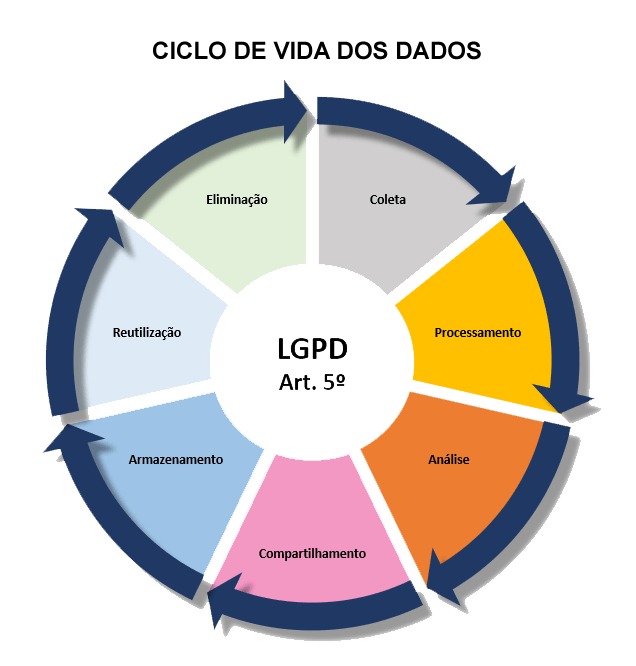
\includegraphics[width=4.3in]{Images/01CicloDeVida.png}
    \label{fig: 01CicloDeVida}
    
    \centering \small Fonte: Xpositum consultória empresarial.
\end{figure}

%02-02-06-03-Revisto[OK]
Antes da existência da LGPD, o ciclo de vida de um dado não necessariamente deveria cumprir certos requisitos de segurança, ocorrendo erros que podiam comprometer a segurança do dado caso utilizado indiscriminadamente. Entretanto, com o surgimento da LGPD, rompe-se com esses possíveis erros. Surgem novos requerimentos legais, como a necessidade de utilizar mecanismos de segurança, adotando desde a sua concepção até o fim da vida de um dado, e também utilizando criptografia, controles e níveis de acesso aos dados, e mecanismos de autenticação \cite{Castro2020}, garantindo a segurança e a integridade em todo o ciclo de vida do dado e da informação \cite{Jimene2020}.

%02-02-06-04-Revisto[OK]
A figura do quadro ilustrativo feito pela Xpositum consultória, elucida na figura \ref{fig: 02CicloDeVida}, o efeito que a LGPD trouxe de antes e depois das fases de ciclo de dados:
\begin{figure}[ht]
    \centering
    \caption{Análise do antes e depois da LGPD.}
    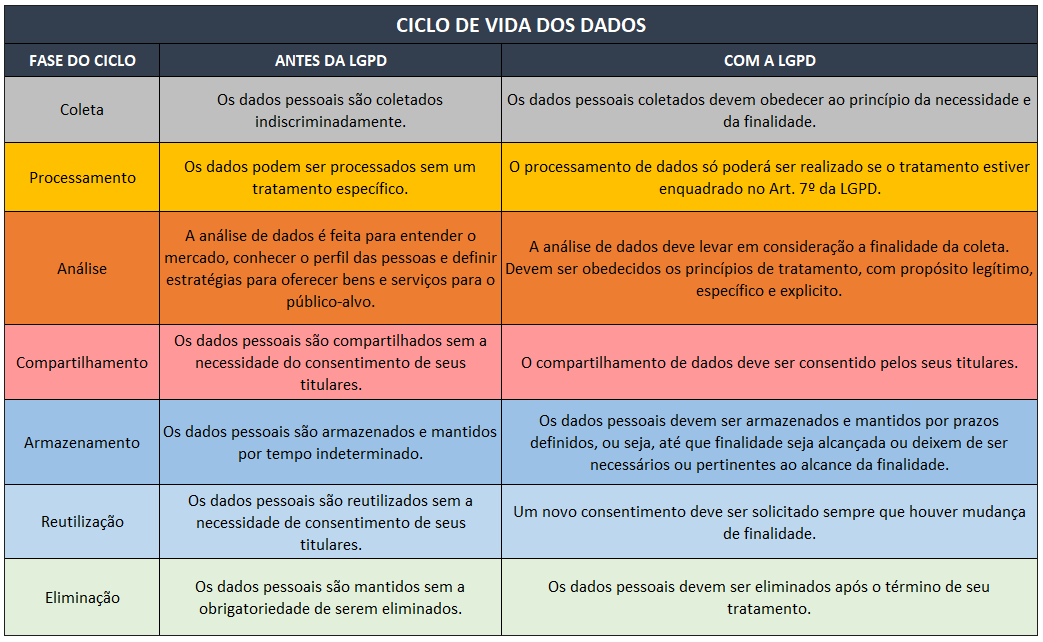
\includegraphics[width=6.2in]{Images/02CicloDeVida.png}
    \label{fig: 02CicloDeVida}
    
     \centering \small Fonte: Xpositum consultória empresarial.
    
\end{figure}

%02-02-06-05-Revisto[OK]
Conforme descrito por \citeonline{Lima2020}, é importante que a organização controladora ou operadora dos dados tenha viés de sempre respeitar o ciclo de vida de um dado, atrelado a necessidade de estar em conformidade. Entender e documentar o ciclo de vida dos dados da organização é vital para o processo de adequação. Configurando-se necessário saber quem são os envolvidos com acesso aos dados durante a fase de processamento, e se essas pessoas possuem conhecimento de suas obrigações e responsabilidades para corresponder com a referida lei \cite{Donda2020}.


% %%%%%%%%%%%%%%%%%%%%%%%%%%%%%%%%%%%%%%%%%%%%%%%%%%%%%%%%%%%%%%%%%%%%%%%%%%%%%%%%%%%%%%%%%%%%%%%%%%%%%%%%%%%%%
% %                      2.3                         
% %%%%%%%%%%%%%%%%%%%%%%%%%%%%%%%%%%%%%%%%%%%%%%%%%%%%%%%%%%%%%%%%%%%%%%%%%%%%%%%%%%%%%%%%%%%%%%%%%%%%%%%%%%%%
\section{Personas da LGPD}
\label{sec: exemplo2}
%02-03-00-00-Revisto[OK]
Nesta seção serão descritos os principais agentes para consolidação da LGPD, sendo descrito o papel do controlador, operador e encarregado dos dados na implementação e tratamentos de dados. E também, a correlação da ANPD com os demais agentes que lidam com dados pessoais. 

% %%%%%%%%%%%%%%%%%%%%%%%%%%%%%%%%%%%%%%%%%%%%%%%%%%%%%%%%
% %                      2.3.1                            % Fazer
% %%%%%%%%%%%%%%%%%%%%%%%%%%%%%%%%%%%%%%%%%%%%%%%%%%%%%%%%
\subsection{Controlador e operador dos dados}

%02-03-01-01-Revisto[OK]
O controlador dos dados é um dos agentes responsáveis pelo tratamento de dados pessoais. Sua previsão legal está no artigo 5, inciso VI da LGPD, podendo ser exercido por uma pessoa física ou jurídica, de direito público ou privado. Compete a tal agente, as decisões a respeito do tratamento dos dados pessoais \cite{01-01-LeiGeral}. Já o outro agente fundamental para a LGPD é o operador, conforme descreve \cite{Pohlmann2019}, que será exercido por uma pessoa física ou jurídica, que, a mando do controlador, realizará o tratamento dos dados pessoais.

%02-03-01-03-Revisto[OK]
Conforme \citeonline{Donda2020} explica e salienta, que o controlador terá várias atuações. Dentre tais ações, será o previsto no artigo 37 da LGPD, o de manter registro das operações de tratamento de dados pessoais que realizaram, se baseando no legítimo interesse; e o previsto no artigo 48 de comunicar a ANPD e ao titular a ocorrência de incidente de segurança que possa acarretar risco ou dano relevante aos titulares \cite{01-01-LeiGeral}. 

%02-03-01-02-Revisto[OK]
O Guia de Boas Práticas da LGPD (2020), traz um exemplo prático e lúcido a respeito do controlador. O exemplo é o de um profissional médico, que armazena os dados pessoais de seus pacientes no computador do consultório. Neste exemplo, o médico será o controlador dos dados pessoais, cabendo-lhe seguir todos os trâmites legais para a proteção de dados pessoais e de saúde dos seus pacientes.

De tal modo, o referido guia de boas práticas, situa também o papel de elaborar o relatório de impacto à proteção de dados pessoais, previsto no artigo 38 da referida lei, tendo também o papel de fornecer informações referentes ao tratamento, assegurar correções e eliminação de dados se respaldando do direito dos titulares conforme o artigo 18 (BRASIL, 2020).
\pagebreak


%02-03-01-04-Revisto[OK]
Já o operador de dados será exercido por uma pessoa física ou jurídica, que a mando do controlador, realizará o tratamento dos dados pessoais, previsto legalmente no artigo 5º, inciso X e também o artigo 39 da LGPD. O operador somente poderá tratar os dados para a finalidade estabelecida pelo controlador, pois o poder de decisão pertence ao controlador, de modo que o operador também deverá manter os registros das operações de tratamentos de dados que realizou \cite{01-01-LeiGeral}.

%02-03-01-05-Revisto[OK]
De modo a sintetizar a LGPD, os autores \citeonline{Blum2020} elencaram uma tabela \ref{tab: responsabilidades do controlador} relacionando as principais atividades exercidas pelo controlador com os artigos e tópicos, conforme estruturado abaixo:

\begin{table}[ht]
    \centering
    \caption{ Responsabilidades do controlador de dados.}
    \label{tab: responsabilidades do controlador}
    \begin{tabular}{|p{4 cm}|p{11.5cm}|p{0cm}|} 
        \hline

        \textbf{Artigo da LGPD} & \textbf{Principais responsabilidades do controlador}  \\ \hline

Art. 6º, X
&
\begin{tabitemize}
\item Identificação do responsável pelo preenchimento;
\end{tabitemize}\\ \hline
Art. 9º, I a V
&
\begin{tabitemize}
\item Finalidade específica do tratamento;
\item Forma do tratamento;
\item Duração do tratamento;
\item Identificação do controlador inclusive as informações de contato;
\item Informações acerca do uso compartilhado de dados pelo controlador e a finalidade do compartilhamento;
\end{tabitemize} \\ \hline
Arts. 7º, 11 e 14
&
\begin{tabitemize}
\item Identificar qual a base legal atribuída a cada operação;
\end{tabitemize}\\ \hline

Capítulo V
&
\begin{tabitemize}
\item Informações relacionadas a transferência internacional, se houver;
\end{tabitemize}\\ \hline

Art. 48º, §1º, I e II
&
\begin{tabitemize}
\item A natureza dos dados pessoais afetados;
\item As informações sobre os titulares envolvidos;
\end{tabitemize}\\ \hline

 
    \end{tabular}
    \newline \newline Fonte: Adaptado de \citeonline{furtado2020}.
\end{table}

%02-03-01-06-Revisto[OK]
Há complexidades na identificação e diferenciação do controlador para o operador, com responsabilidades semelhantes em relação a ambos, existindo uma lacuna na LGPD \cite{Alves2020}. Para facilitar a diferenciação dos papéis, em 2019, o \textit{European Data Protection Supervisor} (EDPS) publicou um guia para definir os papéis e consultas desses agentes. 

%02-03-01-07-Revisto[OK]
O controlador terá maiores responsabilidades, em contrapartida, o operador atuará subordinadamente, respeitando as decisões proferidas pelo controlador. Conforme o artigo 42 da LGPD, ambos têm responsabilidade solidária aos danos causados em decorrência do tratamento irregular \cite{01-01-LeiGeral}. 

Baseando-se nas informações obtidas em \cite{Alves2020}  foi construído a tabela \ref{tab: Diferenças entre controlador e operador}, com as responsabilidades exclusivas do controlador, e as atividades e tarefas de são responsabilidade do operador ou do controlador, conforme abaixo:

\begin{table}[ht]
    \centering
    \caption{Diferenças entre Controlador \textit{versus} Operador}
    \label{tab: Diferenças entre controlador e operador}
   % \textbf{Diferenças entre controlador e operador.}  \\ 

    \begin{tabular}{|p{4 cm}|p{11.5cm}|p{0cm}|} 
        \hline

Controlador: papéis e tarefas de responsabilidade exclusivas 
&
\begin{tabitemize}
\item o controlador decide realizar o tratamento dos dados pessoais ou solicita que outro o faça, que no caso poderá ser o encarregado;
\item o controlador indica operador para o tratamento de dados em seu nome;
\item o controlador decide a finalidade do tratamento;
\item o controlador possui relação direta com os titulares dos dados;
\item o controlador indica o encarregado pelos dados (DPO);
\end{tabitemize}\\ \hline

Controlador e operador: responsabilidades similares
&
\begin{tabitemize}
\item Adotar medidas de segurança, técnicas e metodologias administrativas e tecnológicas aptas a proteger os dados pessoais de acessos não autorizados, fornecendo logs de acesso, e de lidar com situações que envolvam acidentes, destruição, perda, alteração ou qualquer forma de tratamento ilícito, ou inadequado;

\item Estabelecer regras e metodologias de boas práticas, considerando os princípios basilares da LGPD, e formas de garantir a segurança e integridade dos dados pessoais dos titulares;

\item Garantir aos titulares com exatidão e clareza como os dados estão sendo tratados, e fornecer de forma facilitada e gratuita quando o titular exigir informações a respeito dos dados armazenados;

\item Impossibilitar a realização do tratamento para fins discriminatórios, e de modo a prevenir danos em virtude do tratamento de dados pessoais;

\end{tabitemize}\\ \hline
 
    \end{tabular}
    \newline \newline Fonte: Adaptado de \citeonline{Alves2020}.
\end{table}

%02-03-01-08-Revisto[OK]
O Guia de Boas Práticas da LGPD (2020) elucidou o papel de cada agente, apresentando exemplos práticos para elucidar o papel de cada agente envolvido no tratamento de dados. Em um desses exemplos, é de uma empresa de \textit{e-commerce} “XYZ” que será a responsável pela venda de produtos. Neste exemplo, o principal agente será exercido pelo “controlador de dados pessoais”. Entretanto, para o cliente efetuar a compra será necessário o pagamento, que no exemplo dependerá de uma \textit{fintech} “ABC” para fazer a transferência bancária, que terá o papel de operador. De tal modo, não podendo fazer o tratamento de dados fora do que foi orientado, e não podendo utilizar os dados para novos fins que não tenham sido determinados e aceitos pelo controlador.



% %%%%%%%%%%%%%%%%%%%%%%%%%%%%%%%%%%%%%%%%%%%%%%%%%%%%%%%%
% %                      2.3.2                            %
% %%%%%%%%%%%%%%%%%%%%%%%%%%%%%%%%%%%%%%%%%%%%%%%%%%%%%%%%
\subsection{Encarregado dos dados}
%02-03-02-00-Revisto[OK]
Um dos papéis de grande relevância na conjuntura da LGPD é o do Encarregado da Proteção de Dados (EDP). No Brasil, o encarregado também é conhecido popularmente pela sigla inglesa \textit{DPO} originária de \textit{Data Protection Officer}. O encarregado terá o papel de ser responsável, pela conexão entre a empresa com a Autoridade Nacional de Proteção de Dados (ANPD), e de igual modo com os titulares de dados, dentre outras atividades, conforme o artigo 5.º, inciso VIII da LGPD \cite{Basan2021}. 

%02-03-02-01-Revisto[OK]
No programa de implementação da LGPD, o encarregado terá não somente as responsabilidades descritas acima, mas também o de fazer a empresa entrar em \textit{compliance} com as normas, princípios, padrões e principalmente com os artigos da LGPD. Os conhecimentos em ferramentas, técnicas e metodologias que respeitem os princípios da proteção de dados e outras funções serão importantes para as \textit{soft skills} do encarregado \cite{Vainzof2020}.

%02-03-02-02-Revisto[OK]
O Encarregado de Proteção de Dados tem sua base legal no artigo 41 da LGPD, indicado pelo controlador da empresa. De tal modo, é necessário que a identidade e as informações do encarregado sejam divulgadas publicamente, de forma clara e objetiva no site do controlador\cite{Bioni2020}. 

O perfil específico para a função de encarregado não é descrito na LGPD, de modo que poderá ser exercido por profissional de qualquer área, podendo ser um advogado, contador, profissional de T.I, etc. Entretanto, é desejável que tenha conhecimento aprofundado em tecnologia e direito digital, e sempre se aperfeiçoando em novos conhecimentos a respeito de proteção de dados e segurança digital \cite{Pohlmann2019}.

%02-03-02-01-Revisto[OK]
Não sendo necessário conforme nos diz \citeonline{Vainzof2020} o encarregado ter vínculo trabalhista com a empresa, podendo ser desempenhado por um terceirizado, pessoa física ou jurídica.  É importante para o papel do encarregado estar presente e atuando ativamente nas decisões de gestão da empresa em relação aos dados pessoais.

%02-03-02-01-Revisto[OK]
Conforme descrevem os autores \citeonline{Ana2019}, o encarregado terá várias tarefas e funções importantes, dentre elas elencadas na lista abaixo:


\begin{itemize}
\item Estabelecer comitês de privacidade, políticas de privacidade, treinamentos, políticas de relacionamento com fornecedores e públicos, verificando as normas internas e externas;
\item Sendo o porta-voz da empresa, aceitar reclamações e comunicações dos titulares, prestando esclarecimentos e adotando providências;
\item Comunicar a ANPD de possíveis incidentes como vazamento de dados, invasões, etc.; 
\item Cooperar com a ANPD sempre que for solicitado;
\item Criar ações educativas;
\item Estabelecer mecanismos internos de supervisão e de redução de riscos;
\item Monitora conformidade das atividades de tratamentos de dados pessoais com a regulamentação e normas vigentes;
\item Ter feito a realização dos relatórios de impacto à proteção de dados e demais documentações necessárias.
\end{itemize}


% %%%%%%%%%%%%%%%%%%%%%%%%%%%%%%%%%%%%%%%%%%%%%%%%%%%%%%%%
% %                      2.3.3                            %
% %%%%%%%%%%%%%%%%%%%%%%%%%%%%%%%%%%%%%%%%%%%%%%%%%%%%%%%%

%02-03-03-01-Revisto[OK]

\subsection{ANPD}

A Autoridade Nacional de Proteção de Dados (ANPD) é um órgão da administração pública responsável pela fiscalização e comprimento da LGPD. Surgiu com base legal no artigo 55-A, criando a ANPD, com o objetivo de trazer estabilidade e segurança para a aplicação LGPD \cite{Pinheiro2021}.

Segundo os autores \citeonline{02-01-Vainzof2020} a ANPD tem mais de 40 previsões legais dentro da LGPD para diversas finalidades. As principais competências serão previstas no artigo 55-J, onde a ANPD é responsável por vigiar, monitor, solicitar ao controlador ou encarregado o relatório de impacto à proteção de dados e principalmente fiscalizar o cumprimento da LGPD, caso a empresa descumpra a legislação da LGPD, a aplicação de multa poderá chegar até 50 milhões de reais pelas infrações contrárias à lei \cite{Motta}.  

Em \citeonline{Pohlmann2019}, descreve também outras competências, como a de aplicar sanções e elaborar diretrizes para política nacional de proteção de dados pessoais e privacidade. Terá a função de criar padrões normativos, guias informativos \cite{LGPD12Magalhaes2020} baseando-se em técnicas de medidas de segurança, receber as comunicações de incidentes envolvendo dados pessoais, responsável do governo por cuidar que os direitos dos titulares sejam mantidos e respeitados \cite{Gutierrez}.

Para o sucesso da efetividade e aplicação da LGPD em território brasileiro, conforme salientado em \citeonline{Pinheiro2021} é necessário e fundamental dentre suas funções que a ANPD atenda as diversas partes interessadas, desde o titular dos dados, passando pelos entes privados e públicos, alinhando-se aos três poderes Executivo, Judiciário e Legislativo.

Segundo \citeonline{Doneda2020},  o modelo ideal para a ANPD seja que independente, tanto financeiramente, tanto pelas suas decisões, sendo única, central, e formada internamente por um corpo técnico com conhecimento tecnológico, econômico, administrativo, jurídico e de negócios.

Conforme descrito em seções anteriores, o encarregado, deve ser o canal de comunicação entre a ANPD, o controlador, e principalmente os titulares dos dados, responsável por comunicar ao órgão competente e aos titulados dados a ocorrência de incidente de segurança que possa acometer riscos ou danos aos titulares, adotando providências e recebendo comunicações da ANPD, \cite{LGPD12Mag2020}, conforme a figura \ref{fig: Fluxo }.
\begin{figure}[ht]
    \centering
    \caption{Infográfico de comunicação da LGPD entre os agentes}
    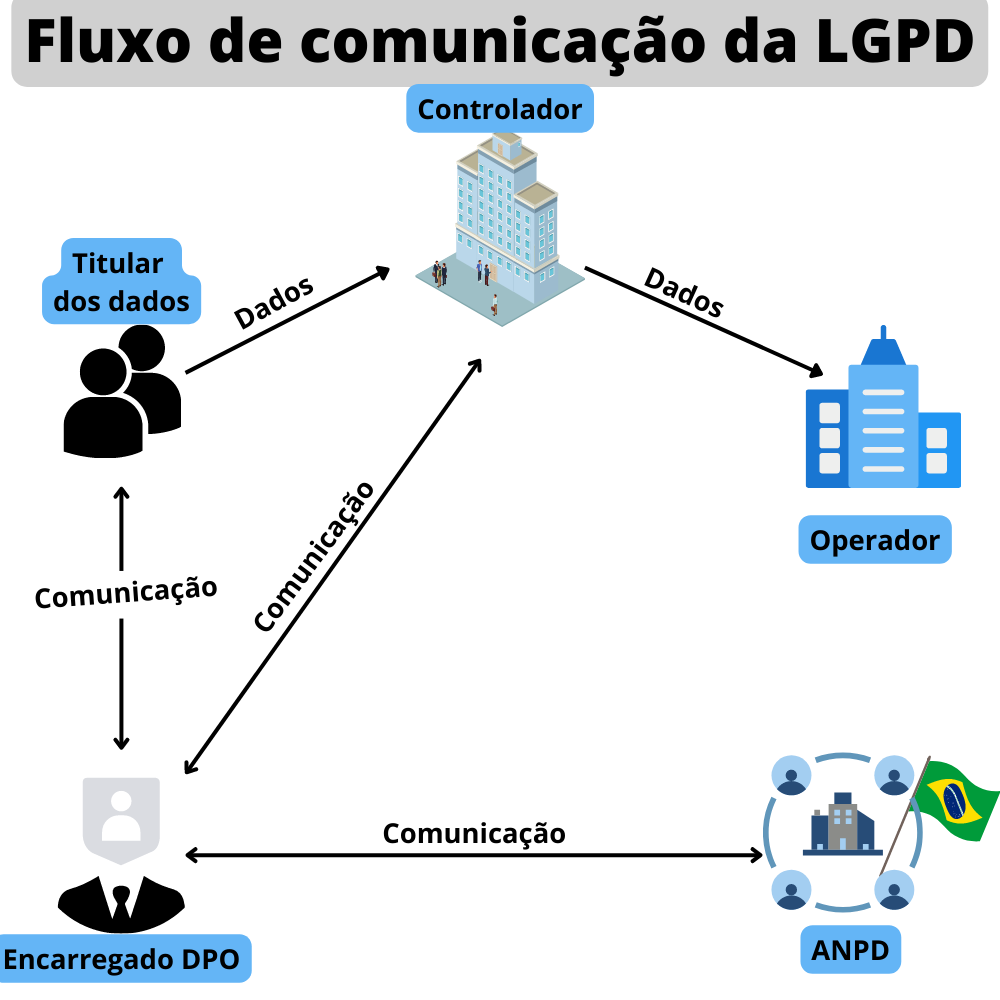
\includegraphics[width=3.0in]{Images/04FluxoLGPD.png}
    
    \label{fig: Fluxo }
    \centering \small Fonte: Autor.
\end{figure}


% %%%%%%%%%%%%%%%%%%%%%%%%%%%%%%%%%%%%%%%%%%%%%%%%%%%%%%%%
% %                      2.4                            %
% %%%%%%%%%%%%%%%%%%%%%%%%%%%%%%%%%%%%%%%%%%%%%%%%%%%%%%%%
\section{A importância da segurança da informação }

De acordo com Sêmola (2003, p. 45), o termo "informação" refere-se a um conjunto de dados utilizados para transferir mensagens entre indivíduos ou máquinas em processos comunicativos. Por sua vez, a segurança da informação é uma área do conhecimento dedicada à proteção dos ativos da informação contra acessos não autorizados, alterações indevidas ou indisponibilidade.

Para garantir essa proteção, a segurança da informação estabelece regras que abrangem todo o ciclo de vida da informação, desde o armazenamento até o descarte, passando pela transferência, manuseio e demais processos. O objetivo é identificar e controlar ameaças e vulnerabilidades que comprometam a integridade, confidencialidade e disponibilidade das informações.

O autor \citeonline{Weidman2014} nos diz que um dos objetivos de um programa de segurança da informação é preservar os três princípios básicos, sendo necessário definir o que é necessário para preservar o nível desejado dos princípios de confidencialidade, integridade e disponibilidade dos sistemas de T.I e dos dados de uma empresa. De modo que o autor \citeonline{Semola2003} elenca o conceito desses princípios:

\begin{itemize}
\item Confidencialidade: é um princípio que significa que toda informação deve ser protegida conforme o grau de sigilo de seu conteúdo, visando a limitação de seus acesso e uso apenas às pessoas para quem elas são destinadas;
\item Integridade: tem o significado que toda informação deve ser mantida na mesma condição que ela foi disponibilizada pelo seu proprietário, visando protegê-las contra alterações indevidas, intencionais ou acidentais;
\item Disponibilidade: por fim, esse princípio significa que toda informação gerada ou adquirida por um indivíduo, ou instituição deve estar disponível aos seus usuários no momento em que os mesmos necessitem para qualquer finalidade.
\end{itemize}

Quando bem implementado, o programa de segurança da informação se torna a defesa contra vulnerabilidades, ataques de \textit{crackers} e \textit{hackers}, e riscos de vazamentos. Conforme afirma Sêmola (\textit{op. Cit.}), tais desafios são constantes e as empresas, independentemente de seus processos, ativos físicos, tecnológicos ou humanos, são sempre alvos de ameaças que procuram lacunas e se aproveitam de vulnerabilidades.

% %%%%%%%%%%%%%%%%%%%%%%%%%%%%%%%%%%%%%%%%%%%%%%%%%%%%%%%%
% %                      2.4.1                            %
% %%%%%%%%%%%%%%%%%%%%%%%%%%%%%%%%%%%%%%%%%%%%%%%%%%%%%%%%

\subsection{Cenário da segurança da informação no Brasil}

A era digital, trouxe muitas vantagens para a sociedade, como a comunicação rápida e dinâmica entre pessoas, podendo a pessoa se comunicar de qualquer lugar do mundo com outras pessoas. Também permitiu a de buscar conhecimento de forma facilitada, sendo que num piscar de olhos pode se ter acesso a inúmeros conhecimentos e comodidades, como poder assistir um filme sem ter que sair de casa, fazer transferências de forma rápida, sem a necessidade de ir em um banco físico, e inúmeras facilitações que a inovação permite a quase todos.

Porém, a era digital trouxe suas desvantagens, como a desigualdade tecnológica, e também o número de golpes, crimes virtuais, ataques cibernéticos, e outros riscos que aumentam de forma exponencial (OLHAR DIGITAL, 2020). As ameaças são incidentes que comprometem a instabilidade das informações, utilizando de exploração de vulnerabilidades, tendo como causa e efeito impactos diretos e indiretos aos negócios da organização.

De acordo com um artigo publicado no site Combate à Fraude (2020), durante o primeiro trimestre de 2020, período em que a pandemia de COVID-19 surgiu, o Brasil foi um dos cinco países mais afetados por fraudes digitais. Além disso, no decorrer do ano de 2020, houve um aumento significativo no número de crimes digitais no país, impulsionado pelo auxílio emergencial e pela introdução do sistema de pagamento PIX do \textit{Open Banking}, o que permitiu que fraudadores explorassem essas novas formas de transação financeira para cometer golpes e enganar vítimas, conforme relata a matéria do G1 (2020).

O site Psafe, especializado em cibersegurança, projetou que em 2021 a quantidade de brasileiros vítimas de phishing seria em torno de 150 milhões (PSAFE, 2021). Com esses números alarmantes e a frequente incidência de golpes e crimes cometidos através da engenharia social, falhas e vazamentos de dados, muitas pessoas continuam sofrendo diariamente nas mãos de criminosos digitais.

No Brasil, existe a necessidade do crescimento de políticas de segurança da informação, tanto para prever criminosos em solo nacional, quanto para precaver de guerras cibernéticas. Atualmente, o Brasil possui um Programa Estratégico de Defesa Cibernética, estruturado pelo Exército brasileiro, e também o decreto nº 9637/2018, que foi posteriormente alterado pelo decreto nº 10.641/2021 que é a Política Nacional de Segurança da Informação (PNSI), abrangendo defesa cibernética, segurança cibernética, segurança física e a proteção de dados organizacionais. (BRASIL, 2021).

% %%%%%%%%%%%%%%%%%%%%%%%%%%%%%%%%%%%%%%%%%%%%%%%%%%%%%%%%
% %                      2.5                            %
% %%%%%%%%%%%%%%%%%%%%%%%%%%%%%%%%%%%%%%%%%%%%%%%%%%%%%%%%
\section{Mecanismos de implementação da conformidade da LGPD}

Neste trabalho será realizada a utilização de um \textit{framework} conceitual, aplicando as técnicas desenvolvidas em empresas, validando a eficiência, e permitindo a reutilização em outros tipos de empresa. Também serão replicados e reutilizados outros \textit{frameworks} como a família série \textit{ISO}, o PCDA, e demais mecanismos para implementação da LGPD. 
% %%%%%%%%%%%%%%%%%%%%%%%%%%%%%%%%%%%%%%%%%%%%%%%%%%%%%%%%
% %                      2.5.1                           %
% %%%%%%%%%%%%%%%%%%%%%%%%%%%%%%%%%%%%%%%%%%%%%%%%%%%%%%%%
\subsection{Conceito de \textit{Framework}}

Conforme descreve \cite{Kechi2012} \textit{framework} é uma arquitetura de processos que podem ser reutilizados e modificados, sendo uma conjuntura de bibliotecas e componentes, com a função de serem utilizados para desenvolvimento rápido e seguro das aplicações. Um \textit{framework} auxilia na agilidade da criação de padrão de projetos, componentes de \textit{softwares}.

Os benefícios de se utilizar ou criar \textit{frameworks} para implementação da proteção de dados está no reuso, na agilidade e na possibilidade de replicar nos projetos de gestão. Em \citeonline{Sommerville2011}, diz a respeito do conceito de \textit{frameworks} “dão suporte ao reuso de projeto, bem como ao reuso de classes específicas de sistema, pois fornecem uma arquitetura de esqueleto para a aplicação. A arquitetura é definida por classes de objetos e suas interações.” 

Conforme \citeonline{Silva2021} os principais tipos de \textit{frameworks} se dividem em: \textit{framework} conceitual que auxilia a identificar itens relevantes e interessantes no domínio da aplicação que apresentam um formato visual de futuros sistemas. Já o \textit{framework} de projetos auxilia na transformação do modelo do domínio da aplicação em um projeto técnico, apresentando um conjunto de padrões ou por estilos de arquitetura. Por fim o \textit{framework} de \textit{software} tem sua utilização na construção e implementação de sistemas computacionais de tamanhos variados, podendo ser de pequena ou média escala.
% %%%%%%%%%%%%%%%%%%%%%%%%%%%%%%%%%%%%%%%%%%%%%%%%%%%%%%%%
% %                      2.5.2                           %
% %%%%%%%%%%%%%%%%%%%%%%%%%%%%%%%%%%%%%%%%%%%%%%%%%%%%%%%%

\subsection{\textit{ISO 27000}: \textit{Framework} de políticas de segurança da informação}

A série de \textit{ISO} 27000 foi criada e desenvolvida pela Organização Internacional de Padrões, fornecendo um \textit{framework} de segurança da informação, podendo ser aplicada em qualquer organização, independente do setor ou tamanho \cite{Pohlmann2019}.

Em breve análise, a \textit{ISO} 27001:2013 define os requisitos a serem atendidos pelo Sistema de Gerenciamento da Segurança da Informação, podendo a organização obter certificação por meio da auditoria e a \textit{ISO} 27002:2013, é tida como guia e manual de boas práticas para controle de segurança da informação, auxiliando na implementação de Sistema de Gestão de Privacidade da Informação (SGPI), \cite{Jimene2020}. Para elucidar de forma fácil, a série de \textit{ISO} 27000 abaixo uma figura \ref{fig: Iso } elencando todas as normas \textit{ISO}.

\begin{figure}[ht]
    \centering
    \caption{Série de \textit{ISO} 27000}
    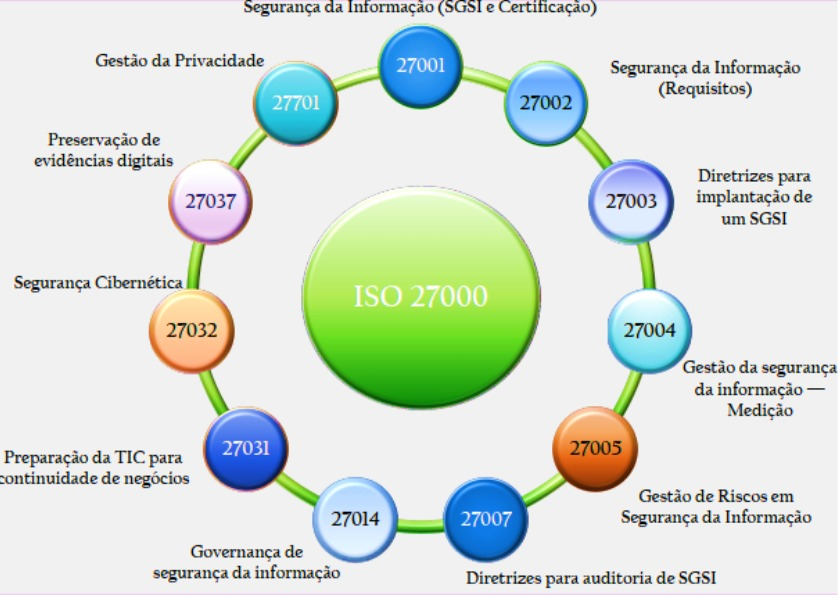
\includegraphics[width=6.0in]{Images/03ISO.jpeg}
    
    \label{fig: Iso }
    \centering \small Fonte: ISACA BH Chapter Elaborado por Fernando Fonseca..
\end{figure}

% %%%%%%%%%%%%%%%%%%%%%%%%%%%%%%%%%%%%%%%%%%%%%%%%%%%%%%%%
% %                      2.5.3                           %
% %%%%%%%%%%%%%%%%%%%%%%%%%%%%%%%%%%%%%%%%%%%%%%%%%%%%%%%%
\subsection{ABNT NBR \textit{ISO/IEC} 27701 }

A norma ABNT NBR \textit{ISO/IEC} 27701:2019 é referente a implementação, manutenção e melhoria contínua de um Sistema de Gestão de Privacidade da Informação (SGPI), sendo a extensão das ABNT NBR ISO/IEC 27001:2013 e ABNT NBR ISO/IEC 27002:2013 para gestão de privacidade \cite{abnt}.

A \textit{ISO} 27701:2019 estabelece critérios e fornece ferramentas para as empresas implementarem a SGPI.  Sendo uma extensão para entrar em conformidade com a LGPD, como os itens que remetem ao artigo 50 da LGPD, que falam sobre boas práticas e governança, visto que, a LGPD não dispõe de maiores detalhes acerca dos requisitos técnicos de segurança a serem adotados na relação controlar e o operador \cite{lgpd1alves}. 

 Pode se citar como alguns dos principais itens dessa \textit{ISO} 27701:2019, conforme também \cite{Vainzof2020}, demonstram:
\begin{itemize}
\item Item 7.2.1: A organização deve identificar e documentar os propósitos específicos pelos quais os dados pessoais são tratados;
\item Item 7.2.2: A organização deve identificar as bases legais pertinentes ao tratamento de dados pessoais;
\item Item 7.2.3: A organização deve determinar e documentar um processo pelo qual possa demonstrar, quando e como o consentimento para o  tratamento de dados pessoais foi obtido;
\item Item 7.2.5: A organização deve avaliar as atividades que geram riscos aos titulares para identificar e realizar relatório de impacto, quando necessário;
\item Item 7.2.8: A organização deve determinar e manter de maneira segura os registros necessários ao suporte às suas obrigações para o tratamento de dados pessoais, demonstrando o tipo de tratamento, propósitos para o tratamento, relatório de Avaliação de Impacto de Privacidade, etc.
\end{itemize}

% %%%%%%%%%%%%%%%%%%%%%%%%%%%%%%%%%%%%%%%%%%%%%%%%%%%%%%%%
% %                      2.5.4                           %
% %%%%%%%%%%%%%%%%%%%%%%%%%%%%%%%%%%%%%%%%%%%%%%%%%%%%%%%%
\subsection{ \textit{PDCA} }

Conforme consolida \citeonline{ALima2020}, a gestão de risco cibernético se baseia em alguns pilares, como: identificar, proteger, detectar e responder e recuperar. A \textit{ISO} 27001 é constituída pelo processo PDCA, que se resume em \textit{Plan} (planejar os controles); \textit{Do} (implementar esses controles); \textit{Check} (checar os controles); \textit{Act} (agir, atualizando os controles, caso na etapa de verificação falhem).

A implementação da LGPD tem várias etapas e processos, e o PCDA conforme demonstra o \textit{website} \cite{minutoseguraca}, pode ser utilizado para simplificar a tarefa de conformidade. Em etapas em relação a LGPD, pode se dividir em 4 fases, que serão contínuas e forma de ciclo, conforme a figura \ref{fig: PCDA }:

\begin{figure}[ht]
    \centering
    \caption{Ciclo PCDA da LGPD.}
    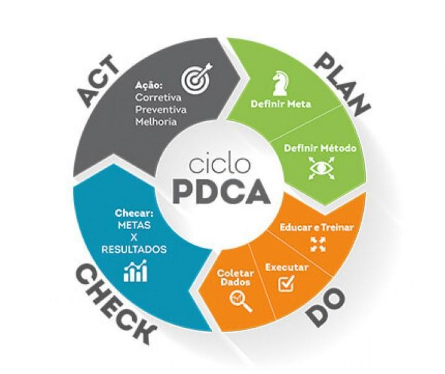
\includegraphics[width=4.2in]{Images/05PCDA.png}
    
    \label{fig: PCDA }
    \centering \small Fonte: Site Oobras.com.br \cite{oobras}.
\end{figure}

\begin{itemize}
\item Fase I  \textit{Plan} — Planejar: essa é uma das fases importantes para o processo de conformidade, visto que deve se identificar os problemas, estabelecer os objetivos e metas, e planejar próximos passos. Conforme o site \citeonline{minutoseguraca}, deve-se analisar de início os 7 princípios da LGPD relacionados ao processo de dados, e também definir os objetivos no tratamento de dados.
\item Fase II \textit{Do} — Executar: será colocar em prática os planejamentos da etapa anterior. Executando utilizando tecnologias para auxiliar a implementação como \textit{frameworks}.
\item Fase III \textit{Check} — Checar: Nesta etapa será de verificar se os trabalhos realizados nas etapas anteriores, verificando se estão sendo executados conforme o planejado. Nessa fase, o autor demonstra a importância de validar através do relatório de impactos a proteção de dados.
\item Fase IV \textit{Act} — Agir:  essa última fase será para corrigir processos que tenham desviado do que foi planejado, investigar as causas e tomar ações em prol de corrigir e melhorar os métodos dos processos. Gerando relatórios e documentações que possam ser úteis para futuras tomadas de decisões.
\end{itemize}

% %%%%%%%%%%%%%%%%%%%%%%%%%%%%%%%%%%%%%%%%%%%%%%%%%%%%%%%%
% %                      2.5.5                           %
% %%%%%%%%%%%%%%%%%%%%%%%%%%%%%%%%%%%%%%%%%%%%%%%%%%%%%%%%
\subsection{ \textit{Privacy by Design}  }

O conceito de \textit{Privacy by Design}, conforme demonstra \cite{oliveira2020}, significa em tradução para o português "privacidade" desde a concepção, e uma das suas principais origens foi através de um artigo da canadense Ann Cavoukian intitulado “\textit{Privacy by Design: The 7 Foundational Principles – Implementation and Mapping of Fair Information Practices}”, \cite{Jimene2020}. Onde ela foi motivada pelos avanços tecnológicos constante, apenas leis não seria o suficiente para garantir a privacidade do usuário. 

A canadense Ann Cavoukian diz que é necessário encorajar as empresas, e todos os envolvidos pela concepção de produtos e serviços, como exemplo desenvolvedores, \textit{designers}, \textit{product} \textit{manager}, etc., a incorporar a privacidade desde o início do projeto, durante a execução até o fim \cite{Vainzof2020}. 

A metodologia \textit{Privacy by Design} criada por Ann Cavoukin trata-se de um \textit{framework}, conforme descreve \citeonline{oliveira2020}. E que a privacidade seja pensada e construída não somente em tecnologias da informação, mas também em práticas de negócios, transformando e fazendo mudanças organizacionais. Modificando o modo de operação padrão de entidades que lidam com produtos ou serviços, com o fim de assegurar que a privacidade seja realizada durante todo o ciclo do tratamento \cite{Ana2019}.

A popularidade desse \textit{framework} tornou-se requisito para conformidade da Regulamento Geral de Proteção de Dados europeia, sendo expresso no artigo 25 do referido  regulamento, que a proteção de dados deve ser desde a concepção e como padrão \cite{oliveira2020}, de modo que aqui no Brasil, a LGPD aplica esse conceito no artigo 46, § 2°, com os seguintes dizeres a respeito das medidas de segurança e proteção de dados: “deverão ser observadas desde a fase de concepção do produto ou do serviço até a sua execução” \cite{01-01-LeiGeral}.

% %%%%%%%%%%%%%%%%%%%%%%%%%%%%%%%%%%%%%%%%%%%%%%%%%%%%%%%%
% %                      2.5.6                           % OK
% %%%%%%%%%%%%%%%%%%%%%%%%%%%%%%%%%%%%%%%%%%%%%%%%%%%%%%%%

\subsection{ RIPD – Relatório de Impacto à Proteção dos Dados Pessoais  }

O Relatório de Impacto à Proteção dos Dados Pessoais (RIPD), também conhecido como DPIA (\textit{Data Protection Impact Assessment}) na GDPR, teve previsão legal no artigo 5º. XVII. É uma das documentações mais importantes que o Encarregado e o controlador de dados pessoais devem elaborar e enviar para a ANPD conforme é dito no artigo 38 da LGPD, \cite{01-01-LeiGeral}.

Para elaborar o RIPD, deve ser instituído e elaborado antes de se iniciar o tratamento dos dados pessoais, conforme elenca o Guia de Boas Práticas (2020), ideal na fase inicial. Conforme a figura elaborada pelo guia, demonstra o ciclo de fases para elaboração do RIPD conforme a figura \ref{fig: CicloRIPD }:
\begin{figure}[ht]
    \centering
    \caption{Ciclo de fases para elaboração do RIPD.}
    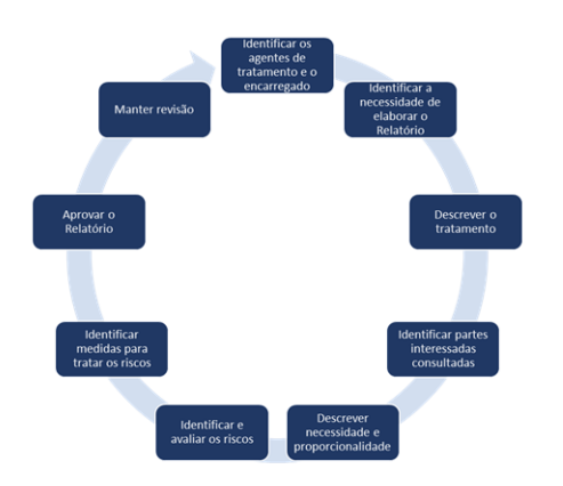
\includegraphics[width=5.5in]{Images/07CicloRIPD.png}
    \label{fig: CicloRIPD }
    
    \centering \small Fonte: Guia de Boas Práticas LGPD (2020)
\end{figure}


%%%%%%%%%%%%%%%%%%%%%%%%%%%%%%%%%%%%%%%%%%%%%%%%%%%%%%%%
%                      Capítulo 3                      %
%%%%%%%%%%%%%%%%%%%%%%%%%%%%%%%%%%%%%%%%%%%%%%%%%%%%%%%%

\chapter{TRABALHOS RELACIONADOS}
\label{ch: trabalhos relacionados}

Neste capítulo são apresentados trabalhos relacionados com o tema de \textit{frameworks} da Lei Geral de Proteção de Dados. Foram utilizados como base de estudos realizados, levando ao entendimento de algumas etapas, conceitos e práticas metodológicas realizadas.

O trabalho de \cite{Blum2020} contribuiu trazendo um trabalho teórico e prático a respeito do papel ativo e suas funções do DPO, o encarregado pelos dados pessoais. Abordando conceitos e ensinamentos para o processo de \textit{compliance} com a LGPD. Conforme os autores salientam, a importância de um marco de privacidade, através de um \textit{framework} é a forma de organizar determinado assunto de forma simples e didática, para possibilitar um melhor controle dos ativos e artefatos, podendo auxiliar na estruturação do programa de conformidade da organização.

A estrutura deste trabalho é sólida, visto que foi constituída por especialistas sobre tecnologia e direito digital. Foram abordados conceitos que contribuíram para a elaboração do \textit{framework} proposto neste trabalho, como os ISOs 27001 e 27701, e do \textit{privacy by design}, e apresentando outros \textit{frameworks} já consolidados no Brasil e mundialmente a respeito de proteção de dados e gestão de riscos, dentre eles se destacam:

\begin{itemize}
\item \textit{Framework} NIST: O National Institute of Standards and Technology  (NIST), é um \textit{framework} de privacidade, com sua abordagem ao gerenciamento de risco à privacidade, se enfatizando, a importância da participação ativa dos cargos mais importantes na instituição, com os colaboradores entendendo sendo informados e treinados \cite{Blum2020}. Dentre outras atribuições que esse \textit{framework} remete aos cinco principais pilares: identificar, proteger, detectar, responder e recuperar; 
\item \textit{OECD Guidelines on the Protection of Privacy and Transborder Flows od Personal Data}: foi criado pela Organização para a Cooperação e Desenvolvimento Econômico (OCDE) visando padronizar e proteger a privacidade no compartilhamento internacional de dados pessoais entre os países membros;
\item \textit{Generally Accepted Privacy Principles} (GAPP): Foi consolidado no Canadá para mensurar a conformidade das organizações referentes ao cumprimento das legislações de proteção de dados do referido país. 

\end{itemize}

%%%%%%%%%%%%%%%%%%%%%%%%%%%%%%%%%%%%%%%%%%%%%%%%%%%%%%%%
%                      Silva    2020               %
%%%%%%%%%%%%%%%%%%%%%%%%%%%%%%%%%%%%%%%%%%%%%%%%%%%%%%%%

A proposta de \citeonline{Silva2020} foi desenvolvido o \textit{framework} para proteção de dados visando implementar dentro de uma instituição de ensino superior. O autor elencou em seu trabalho a governança da tecnologia da informação nas instituições de ensino superior, juntamente trazendo a respeito da estrutura de governança de TI chamada COBIT (Control Objectives for Information and related Technology), na sua versão 5, visando desenvolver ferramentas para fortalecer negócios e a TI, e também os riscos de segurança, como governança de risco e política de risco, elencando a ISO 31000.

Além do \textit{framework}  COBIT 5, o autor elenca outro importante \textit{framework}  que é o COSO-ERM, que possui cinco pilares fundamentais e vinte princípios, tendo o objetivo de facilitar a aplicação para análise e desenvolvimento em atividades de gerenciamento de riscos da organização.

\begin{figure}[ht]
    \centering
    \caption{\textit{Framework COSO-ERM}.}
    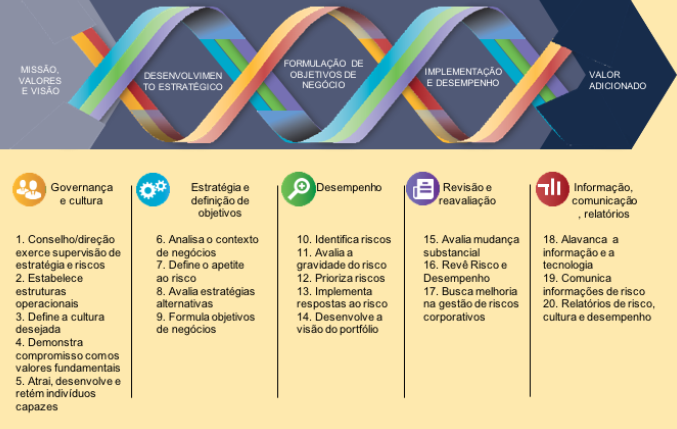
\includegraphics[width=6.8in]{Images/12Silva2020.png}
    \label{fig: 12Silva}
    
    \centering \small Fonte: Blog Riskfence.
\end{figure}

\pagebreak

A metodologia de pesquisa utilizada para a construção do \textit{framework} do autor foi através da elaboração de uma pesquisa intervencionista. Por fim, utilizando das metodologias \textit{COSO}, \textit{COBIT}, \textit{ISO 31000} e a LGPD, o resultado para o plano de adequação esquematizado foi como demonstra a figura \ref{fig: silva2}: 


\begin{figure}[ht]
    \centering
    \caption{Plano de Adequação Esquematizado.}
    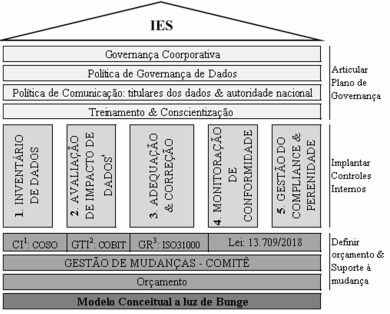
\includegraphics[width=6.0in]{Images/13Silva2020.png}
    \label{fig: silva2}
    
    \centering \small Fonte: \cite{Silva2020}.
\end{figure}

No pensamento de \cite{Silva2020}, a metodologia de avaliação do autor para medir a eficiência do \textit{framework}  foi através da avaliação com questionários. E as fases de adequação do \textit{framework}  proposto pelo autor se dividiu em 5 fases, conforme a imagem \ref{fig: silva3} abaixo: 
\pagebreak

\begin{figure}[ht]
    \centering
    \caption{5 fases do \textit{framework} de (SILVA, 2020) }
    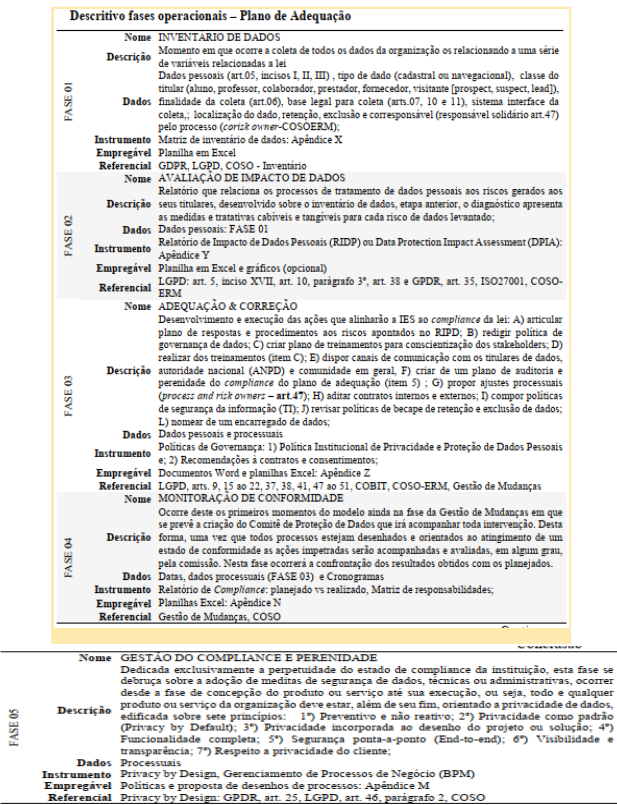
\includegraphics[width=5.6in]{Images/14Silva2020.png}
    \label{fig: silva3}
    
    \centering \small Fonte: (SILVA, 2020).
\end{figure}

\pagebreak

%%%%%%%%%%%%%%%%%%%%%%%%%%%%%%%%%%%%%%%%%%%%%%%%%%%%%%%%
%                      Zini                   %
%%%%%%%%%%%%%%%%%%%%%%%%%%%%%%%%%%%%%%%%%%%%%%%%%%%%%%%%

 Para o \textit{framework}  proposto por \cite{Zini2020} se baseou inicialmente em 3 passos para o tratamento de dados pessoais. Na primeira parte, a autora dividiu em três passos o tratamento de dados pessoais:

\begin{itemize}
\item Identificar nomenclaturas de tratamento de dados: nessa primeira parte, a autora coloca para ao fazer o processo de \textit{compliance} com a LGPD, o primeiro passo seja analisar os principais verbos da lei referentes a tratamento de dados, sendo (acesso, armazenamento, arquivamento, avaliação, classificação, coleta, comunicação, controle, difusão, distribuição, eliminação, extração, modificação, processamento, produção, recepção, reprodução, transferência, transmissão, utilização)
\item Finalidade, clareza e propósitos específicos: nesse passo, a autora enfatiza a importância de se certificar que a operação cumpre sua finalidade e que o titular de dados foi informado claramente e objetiva os propósitos para o tratamento de seus dados.
\item 10 princípios e 10 hipóteses: no terceiro passo, a autora se baseia no artigo 6º que é referente aos 10 os princípios de tratamento de dados e o artigo 7º das hipóteses de tratamento de dados pessoais.
\end{itemize}

Na segunda parte do \textit{framework} , a autora elenca os riscos envolvidos devido a não adequação a LGPD, presentes no artigo 52 da LGPD, sendo que, ela elencou alguns dos riscos para o negócio, como é o caso das sanções da LGPD.

Na terceira parte do \textit{framework} , a autora descreve a respeito da mitigação de riscos das empresas, partindo da segurança da informação, descrita de forma esquematizada os principais artigos dentro da LGPD referente a SI, presentes no artigo 6º, 44º, 46 e 47 da LGPD, sendo um ponto de atenção, para que as empresas possam estar atentos e corrigir as mazelas, enfatizando os passos de implementação (preparação, mapeamento, avaliação, planejamento, execução, monitoramento).

O \textit{framework}  proposto pela autora foi baseado em John Latam, cujo objetivo da autora, é cobrir os requisitos e artigos da LGPD, aplicando boas práticas de governança e segurança dos dados, onde o resultado ficou esquematizado da seguinte esquematização:

\begin{figure}[ht]
    \centering
    \caption{\textit{Framework Zini, 2020}.}
    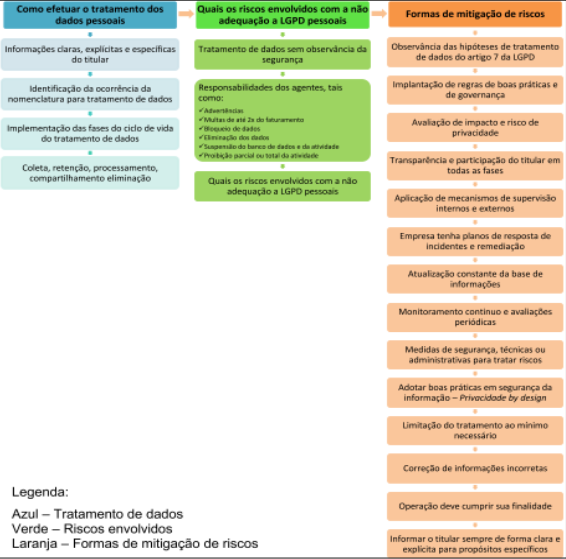
\includegraphics[width=4.9in]{Images/11Zini.png}
    \label{fig: zini}
    
    \centering \small Fonte: \cite{Zini2020}.
\end{figure}

\pagebreak


%%%%%%%%%%%%%%%%%%%%%%%%%%%%%%%%%%%%%%%%%%%%%%%%%%%%%%%%
%                      Carvalho                   %
%%%%%%%%%%%%%%%%%%%%%%%%%%%%%%%%%%%%%%%%%%%%%%%%%%%%%%%%
Em \citeonline{Carvalho2021} foi elaborado o \textit{framework}  baseando-se em um estudo de caso para prevenção a fraude no contexto exclusivo de Big Data, com a proposta de acelerar projetos de \textit{big data} para tratamento de dados voltados à prevenção a fraude em \textit{compliance} à LGPD, utilizando como uma das metodologias o \textit{Design Science Research}.

O \textit{framework}  foi estruturado agregando-se ao ciclo PDCA, dividido em quatro fases principais que se encadeiam que são:

\begin{itemize}
\item Planejamento: Fase inicial, realizadas definições iniciais, como definição de políticas, processos, responsáveis, requisitos, modelos, etc.
\item Desenvolvimento: Tal fase é a implementação dos dados, bases e estruturas, realizado as análises e extração dos dados.
\item Controle: Fase de monitoração e análise das validações, testes e verificações realizadas;
\item Ação: Fase onde é efetuado a análise crítico, buscando melhorias e soluções contínuas.
\end{itemize}

Conforme a figura \ref{fig: Carvalho }, ficou esquematizado como ficou a estrutura do \textit{framework} proposto pelo autor \cite{Carvalho2021}:

\begin{figure}[ht]
    \centering
    \caption{\textit{Framework} elaborado por Carvalho (2021).}
    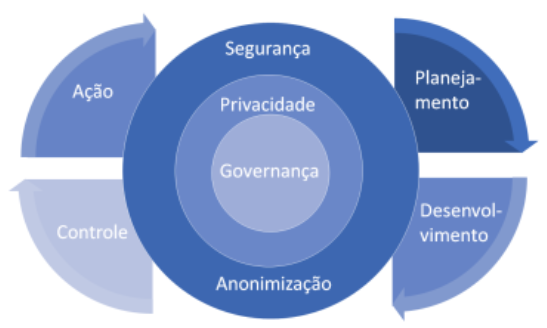
\includegraphics[width=6in]{Images/08Carvalho2021.png}
    \label{fig: Carvalho }
    
    \centering \small Fonte: Carvalho (2021, p. 89).
\end{figure}

Para a efetiva validação do \textit{framework}, o referido autor, utilizou dois projetos de ingestão de dados em Big Data, sendo que no primeiro projeto, a ingestão de dados foi sem observar as boas práticas elaboradas pelo \textit{framework}, e no segundo projeto foi objetivando o \textit{framework}. Para fazer o processamento dos projetos, o autor utilizou da ferramenta \textit{Apache Hadoop}, e por fim extrair métricas de performance.

\pagebreak
%%%%%%%%%%%%%%%%%%%%%%%%%%%%%%%%%%%%%%%%%%%%%%%%%%%%%%%%
%                      Menegazzi                  %
%%%%%%%%%%%%%%%%%%%%%%%%%%%%%%%%%%%%%%%%%%%%%%%%%%%%%%%%
O trabalho de \cite{Menegazzi2021} propõem como \textit{framework}  um guia dividido em 6 etapas para o \textit{compliance} com a LGPD. Sendo durante o trabalho o autor elabora um guia de engenharia de requisitos com as propostas de conformidade, conforme a figura \ref{fig: Menegazzi } abaixo: 

\begin{figure}[ht]
    \centering
    \caption{Engenharia de requisitos do \textit{framework} Menegazzi (2021).}
    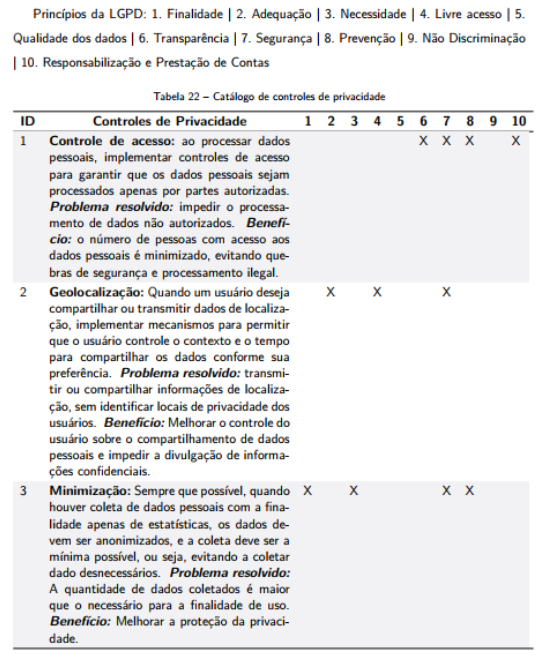
\includegraphics[width=6.3in]{Images/09Menegazzi.png}
    \label{fig: Menegazzi }
    
    \centering \small Fonte: \cite{Menegazzi2021}.
\end{figure}


O autor também descreveu a respeito sobre requisitos de negócios, também denominado como Regras de Negócio, atrelando os referidos requisitos aos princípios e artigos da LGPD, conforme a figura \ref{fig: MenegazziFigB}. Por fim, avaliando o guia proposto, com um questionário de avaliação via Google Forms, respondido por pessoas de diversas áreas, e como resultado do trabalho realizado e também de modo para facilitar a proposta do guia, o autor criou um website com vídeos explicativos e etapas do guia de conformidade.

\begin{figure}[ht]
    \centering
    \caption{Requisitos de negócio do framewok Menegazzi (2021)}
    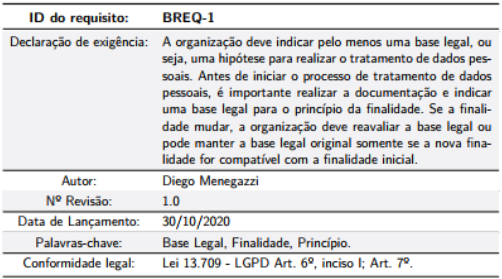
\includegraphics[width=6.5in]{Images/10Menegazzi.png}
    \label{fig: MenegazziFigB}
    
    \centering \small Fonte: \cite{Menegazzi2021}.
\end{figure}



Em \citeonline{Menegazzi2021} divide sua proposta de \textit{framework} em 6 etapas do guia foram divididas conforme as listas abaixo:
\begin{itemize}
\item Auditoria de Dados: É a primeira etapa, onde é realizado o mapeamento inicial dos dados, analisar quais dados a organização está tratando, quais categorias são só dados, se estão sendo compartilhados, como estão sendo armazenados, coletados e manipulados, sendo esse processo realizado através de uma entrevista com o responsável pela manipulação dos dados.
\item Análise de Lacunas: Essa segunda etapa é feita a análise das informações obtidas na primeira etapa, com objetivo de identificar passos como (fluxos, processos, requisitos) que precisam ser melhorados por ações corretivas e/ou preventivas. Também nessa etapa, foi elaborado um questionário para analisar possíveis violações dos princípios da LGPD
\item Planejamento e Preparação: Nesta terceira etapa, o objetivo é solucionar problemas que surgiram na segunda etapa, e para corrigir as violações aos princípios, o autor elabora requisitos de negócio para alterações as violações de princípios, dividido em descrição do problema, problema resolvido e o benefício em resolver o problema. 
\item Revisão do Plano de Ação: Essa quarta etapa, conforme o autor descreve, é importante que os stakeholders revisem o plano de ação elaborado na terceira fase, e se as mudanças impactaram o funcionamento do negócio.
\item Execução: A quinta etapa, as análises sugeridos na quarta etapa, devem estar prontos para que as soluções sejam implementadas. Nesta etapa, é necessário o conhecimento profundo de profissionais como o Encarregado, que deve ter conhecimentos sobre segurança e privacidade, com os demais profissionais da equipe para fazer a implementação.
\item Revisão Pós-implementação: por fim, essa é a última etapa, onde o encarregado e o controlador dos dados deverão garantir que todos os requisitos de conformidade com a LGPD foram atendidos.
\end{itemize}




%%%%%%%%%%%%%%%%%%%%%%%%%%%%%%%%%%%%%%%%%%%%%%%%%%%%%%%%
%                      Silva     2021               %
%%%%%%%%%%%%%%%%%%%%%%%%%%%%%%%%%%%%%%%%%%%%%%%%%%%%%%%%
O autor \citeonline{silva2021}, desenvolveu o \textit{framework} para implementação da LGPD baseando-se inicialmente as leis de privacidade mais populares no Brasil, GDPR, CCPA e LGPD, e outras ISO e \textit{frameworks} existentes, tendo como resultado um \textit{framework} em cinco fases, conforme a figura \ref{fig: silva21} abaixo:

\begin{figure}[ht]
    \centering
    \caption{\textit{Framework 5 fases \citeonline{silva2021} }.}
    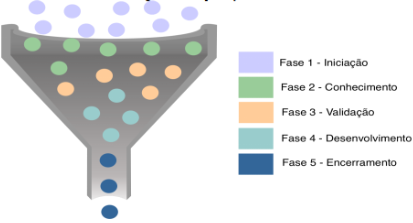
\includegraphics[width=3.8in]{Images/15Silva2021.png}
    \label{fig: silva21}
    
    \centering \small Fonte: \cite{silva2021}.
\end{figure}

\pagebreak

Sendo dividido em 5 fases para implementação da LGPD as seguintes fases: 
\begin{itemize}
\item Iniciação: Nessa primeira fase, o autor elenca a importância do conhecimento da alta gestão da empresa em conhecer o processo de adequação a LGPD, e com o objetivo do conhecimento de todos os colaboradores da empresa, o cargo mais alto, que no caso seria o CEO ou presidente da organização deverá comunicar a empresa e seus colaboradores, e também internamente e externamente sobre o início do processo de adequação. E também a criação de uma carta com o breve histórico da organização, abordando a necessidade de conformidade, e também elencar a equipe responsável pelo plano de conformidade com a LGPD, criando o comitê de governança de dados, e destinando um responsável por ele, tendo o papel contínuo de melhoria.
\item  Conhecimento: Na segunda fase, são feitas análises internas de processos e fluxos de informações e dados na empresa. Analisando como a organização recebe os dados, faz o tratamento e armazenamento, e quem tem acesso a esses dados. Fazendo uma lista para saber como as informações são recebidas e armazenadas, o autor, efetua cinco perguntas principais que são: quem envia informações pessoais para a empresa?; como a empresa recebe dados pessoais?; em cada entrada que categoria de dados pessoais é coletado?; em cada entrada, como é armazenado os dados pessoais?; e por fim, quem tem ou poderia ter acesso aos dados pessoais coletados?; desenhando por fim, um fluxo de dados. Desenvolvendo uma planilha exemplo do levantamento de dados pessoais.
\item Validação: O autor, nessa terceira fase, depende que a segunda fase esteja finalizada para dar prosseguimento ao processo de conformidade. Na fase de validação, o autor desenvolveu um questionário com indagações a serem respondidas a respeito do processamento se está sendo processado de forma justa e legal?; se os propósitos estão especificados, quais as finalidades; a respeito da relevância dos dados, se são relevantes e não tem excesso em relação à finalidade; a precisão dos dados, se os dados se mantêm inviolados; a retenção dos dados, se os dados não são mantidos mais tempo que o necessário; o processamento justo, onde os dados são tratados consoante os direitos dos titulares de dados conforme a LGPD, e por último, a responsabilização, se são tomadas e executadas medidas técnicas e organizacionais para adequação da LGPD contra o processamento não autorizado ou ilegal, e também contra perdas, destruição ou dano de dados pessoais.

\item Desenvolvimento: nessa penúltima fase, as etapas fundamentais que o autor descreve são o de realizar a comunicação e treinamento para todos os colaboradores da empresa em relação à proteção de dados, juntamente com um plano de treinamento interno, contendo a estratégia e o plano de conscientização. Também será nessa fase que serão desenvolvidos a matriz de responsabilidade, as políticas de segurança de dados pessoais, além da importância em documentar os fluxos de dados internos e externos da organização, fluxograma com processos e etapas, e o plano de ações.
\item Encerramento: a última etapa é a consolidação de todas as etapas anteriores, conforme descreve o autor, o resultado obtido é utilizado para a criação do relatório de análise de proteção de dados, com o sistema de fluxo de dados, as políticas de proteção de dados e documentos com o nível de conformidade da organização.
\end{itemize}

Sendo gerado como resultado dos analises levantamentos de requisitos dos dados conforme a figura \ref{fig: silva21A}:

\begin{figure}[ht]
    \centering
    \caption{Levantamentos de Requisitos.}
    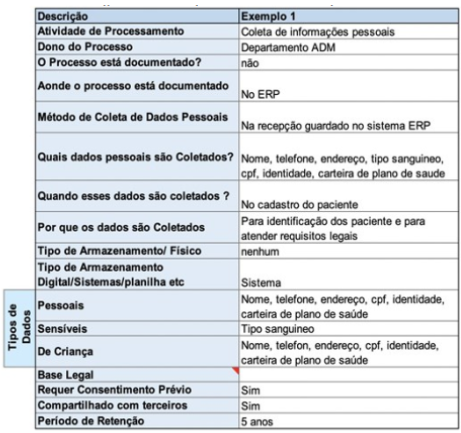
\includegraphics[width=4.3in]{Images/16Silva2021.png}
    \label{fig: silva21A}
    
    \centering \small Fonte: (SILVA, 2021).
\end{figure}

\pagebreak

Como resultado final do \textit{framework}, foi construído um quadro utilizando a metodologia Kanban no Trello, utilizando \textit{cards} com as tarefas a serem realizadas e desenvolvidas. Conforme a imagem abaixo, temos o resultado final do \textit{framework}, onde foi feito a gestão do projeto de conformidade do autor:

\begin{figure}[ht]
    \centering
    \caption{Kanban do \textit{framework} do autor (SILVA, 2021).}
    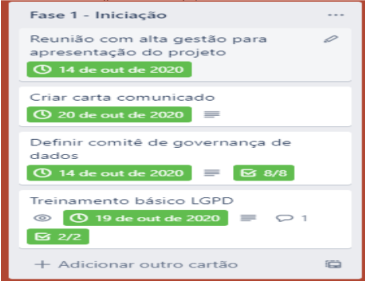
\includegraphics[width=4.0in]{Images/17Silva2021.png}
    \label{fig: grafico-acc}
    
    \centering \small Fonte: \cite{silva2021}.
\end{figure}

Feito o estudo dos trabalhos relacionados que foram uteis para o estudo bibliográfico e construção do \textit{framework}  proposto nesse trabalho, podemos construir um quadro comparativo entre os trabalhos correlatos e o presente trabalho, com os principais diferencias.
\begin{table}[ht]
    \centering
    \caption{Tabela comparativa entre os trabalhos relacionados e o \textit{framework proposto}.}
    \label{tab: requisitos de tratamento de dados}
    \begin{tabular}{|p{5.5 cm}|p{4.5cm}|p{5.5cm}|} 
        \hline
        \textbf{Autor} & \textbf{Dispositivo legal} & \textbf{Requer consentimento?} \\ \hline
        
         Proposta do autor & LGPD, art. 7º, inciso I & Sim \\ \hline
         
        Hipótese 2: Para o cumprimento de obrigação legal ou regulatória & LGPD, art. 7º, inciso II & Não  \\ \hline
        
        Hipótese 9 : Para atender interesses legítimos do controlador ou de terceiro & LGPD, art. 7º, inciso IX & Não  \\ \hline
        
        Hipótese 10: Para proteção do crédito & LGPD, art. 7º, inciso X & Não  \\ \hline
    \end{tabular}
    \newline \newline Fonte: Autor.
\end{table}


%%%%%%%%%%%%%%%%%%%%%%%%%%%%%%%%%%%%%%%%%%%%%%%%%%%%%%%%
%                      Capítulo 4                      %
%%%%%%%%%%%%%%%%%%%%%%%%%%%%%%%%%%%%%%%%%%%%%%%%%%%%%%%%

\chapter{METODOLOGIA}
\label{ch: materiais e métodos}

Neste capítulo, são discutidos os materiais e métodos utilizados ao longo do desenvolvimento deste projeto. Materiais e métodos esses sendo utilizados ferramentas e \textit{softwares} gratuitos que permitiram o bom desenvolvimento e manutenção do presente trabalho.
Nas subseções são apresentados os materiais utilizados, como a modelagem do banco de dados, requisitos de negócios, arquitetura de sistema e a construção do \textit{framework}. A partir de etapas da engenharia de \textit{software} e modelagem de requisitos foram estipulados os diagramas que auxiliaram na construção desse projeto.
Para o desenvolvimento do \textit{software} do \textit{framework} de implementação a LGPD do referido trabalho foi baseado nos conhecimentos adquiridos ao decorrer da graduação de Ciência da Computação.


% %%%%%%%%%%%%%%%%%%%%%%%%%%%%%%%%%%%%%%%%%%%%%%%%%%%%%%%%
% %                      4.1                         %
% %%%%%%%%%%%%%%%%%%%%%%%%%%%%%%%%%%%%%%%%%%%%%%%%%%%%%%%%
\section{Materiais}

A metodologia para a escrita foi através da realização de revisões a respeito da temática e análise por pesquisa bibliográfica. Proveniente de livros, periódicos acadêmicos, e conteúdo em \textit{sites} da \textit{internet}.

Buscando-se por principais trabalhos relacionados a implementação da LGPD, posteriormente dissertações relacionadas ao tema de \textit{framework}  de conformidade da referida lei. Sendo procurado artigos dos anos de 2018 até 2022 nas bases da Capes, Oasis-Br e Google Acadêmico. 

Os artigos e livros encontrados foram analisados e feito o fichamento, posteriormente, classificando quais seriam benéficos para as fundamentações e desenvolvimento deste trabalho.

% %%%%%%%%%%%%%%%%%%%%%%%%%%%%%%%%%%%%%%%%%%%%%%%%%%%%%%%%
% %                      4.2                         %
% %%%%%%%%%%%%%%%%%%%%%%%%%%%%%%%%%%%%%%%%%%%%%%%%%%%%%%%%
\section{Requisitos de negócios}

Conforme descreve \citeonline{Vazquez2016}, requisitos (ou necessidades) de negócios são “declarações de mais alto nível de objetivos, metas ou necessidades da organização”.  Os motivos pelo qual o projeto está sendo iniciado serão descritos neste documento. Visto que, elencado pelo autor, as necessidades de negócios têm o objetivo de resolver problemas ou aproveitar futuras oportunidades, mantendo condições atuais para futuras alterações.

O levantamento de requisitos de negócios foi essencial para elucidar e nortear a viabilidade e ver quais requisitos deveriam ser priorizados no sistema a ser desenvolvido, as partes de regra de negócio, e os requisitos fundamentais e não fundamentais deste trabalho, \cite{Vazquez2016}. Algumas das perguntas elencadas foram:

\begin{itemize}
\item “Quais as principais funções do sistema?”
\item “Qual é o público alvo?”
\item “Quantos atores terá o sistema?”
\item “Quais os requisitos fundamentais?”
\item “Como desenvolver um sistema de boa experiência para o usuário?”
\end{itemize}

Para construção do \textit{framework}  foi realizado a análise da engenharia de requisitos, sendo feitos as regras de negócio, os requisitos funcionais e requisitos não funcionais do sistema \textit{web} proposto. Feito essas análises foi possível ter a visão ampla das usabilidades de cada parte do sistema e documentar para futuras implementações.  As regras de negócio juntamente com os requisitos funcionais e não funcionais estão disponíveis no Github do projeto através do link: \url{https://github.com/felipecandian/TCC-DadosLGPD}.

As regras de negócio têm o objetivo de documentar as regras que são aplicáveis ao negócio e que direcionaram aos casos de uso. Como descreve em \citeonline{Vazquez2016}, as regras de negócio devem ser tratadas como ativo organizacional e em \cite{Wazlawick2013} são declarações e condições que devem ser satisfeitas.

Os requisitos funcionais devem ser descritos os comportamentos que o \textit{software} tem em razão das tarefas ou serviços de usuários. Conforme descrito por Sommerville (2011, p.75), “os requisitos funcionais de um sistema descrevem o que ele deve fazer”. E o mesmo autor descreve que tais requisitos devem fornecer previsões de ações no sistema, como reagir a entradas específicas e se comportar em determinadas situações, também explicando o que o sistema não deve fazer.

Abaixo alguns exemplos de requisitos funcionais do \textit{framework} estão no Github na pasta DOCUMENTAÇÃO e DIAGRAMAS.
\begin{itemize}
\item O sistema não deve permitir acessos não autorizados;
\item O sistema deverá ter hierarquia de acessos;
\item O sistema deve permitir que usuários respondam o questionário.
\end{itemize}

Os requisitos não funcionais, como visto em \citeonline{Sommerville2011} descrevem limitações como relacionadas ao ambiente, como segurança, privacidade e sigilo, a organização, a implementação e por fim, a qualidade. Conforme descrito por Sommerville (2011, p.76) “não estão diretamente relacionados com serviços específicos oferecidos pelo sistema a seus usuários.”. 

Listado abaixo, alguns exemplos de requisitos não funcionais do \textit{framework}:

\begin{itemize}
\item O sistema web deve ser responsivo, permitindo ser utilizado e visualizado em qualquer aparelho móvel;
\item Deve utilizar para armazenamento o banco de dados em \textit{MySQL};
\item O sistema de questionário deve ser feito utilizando \textit{Javascript} e \textit{PHP};
\end{itemize}

% %%%%%%%%%%%%%%%%%%%%%%%%%%%%%%%%%%%%%%%%%%%%%%%%%%%%%%%%
% %                      4.3                         %
% %%%%%%%%%%%%%%%%%%%%%%%%%%%%%%%%%%%%%%%%%%%%%%%%%%%%%%%%
\section{Casos de Uso e Diagrama de casos de uso}

O conceito de caso de uso trata-se de uma modelagem UML (Unified Modeling Language), que serve para documentações  \cite{Sommerville2011}. Sendo conceituado como um conjunto de passos que ilustra um cenário principal e também possíveis cenários para que um ator possa objetivamente usar o sistema. Para Vazquez e Simões (2016, p.399), o diagrama de caso de uso “ilustra graficamente os casos de uso suportados por um sistema, os atores que interagem com estes e os relacionamentos entre os casos de uso e os atores”.

Graficamente o diagrama de caso de uso tem os seguintes elementos básicos, conforme em \cite{Vazquez2016}:

\begin{itemize}
\item Ator: representará uma pessoa ou grupo de pessoas que atuaram com o papel de interagir com o \textit{software}. Podendo o ator ser ativo ou passivo, sendo ativo quando o ator inicia a execução do caso de uso. E será passivo quando o caso de uso não é iniciado pelo autor, reagindo pelas ações do sistema.
\item Caso de uso: será as funcionalidades que atende a um ou mais requisitos do cliente. Como padrão sugere-se a usar os verbos das ações dos casos de uso no infinitivo, sendo representado por uma elipse com a ação escrita.
\item Relacionamento: é quando um ator interage com um caso de uso, representando um relacionamento que podem ser generalização, extensão ou inclusão.
\end{itemize}

A importância de se utilizar os casos de uso na construção de um \textit{software}, está na importância de se documentar e também ajudar no entendimento dos requisitos funcionais do sistema \cite{Fowler2007}. Na construção do caso de uso, primeiramente deve se definir quais eram os conjuntos de autores e como eles se relacionam com o sistema, suas atribuições e funções \cite{Pressman2011}.

Para esse trabalho, o diagrama de caso de uso foi construído pelo \textit{software} Astah, onde foi feito dois atores principais, o \textit{DPO} e a empresa que terá o processo de conformidade. Para acessar as documentações de requisitos e diagramas de casos de uso realizados estão disponibilizados no Github pelo link: \url{https://github.com/felipecandian/TCC-DadosLGPD}.

\pagebreak

% %%%%%%%%%%%%%%%%%%%%%%%%%%%%%%%%%%%%%%%%%%%%%%%%%%%%%%%%
% %                      4.4                         %
% %%%%%%%%%%%%%%%%%%%%%%%%%%%%%%%%%%%%%%%%%%%%%%%%%%%%%%%%
\section{Arquitetura do sistema}

O modelo arquitetural de construção de \textit{software} adotado para o projeto foi o padrão de projeto MVC (Model, View, Controller), em tradução para o português significa: modelo, visão e controlador. Conforme definido por Gamma et al., (2007, p.20), que a respeito do MVC diz:  “Modelo é o objeto de aplicação, a Visão é a apresentação na tela e o Controlador é o que define a maneira como a interface do usuário reage às entradas do mesmo”.

\begin{figure}[ht]
    \centering
    \caption{Arquitetura MVC: Interação entre as camadas MVC.}
    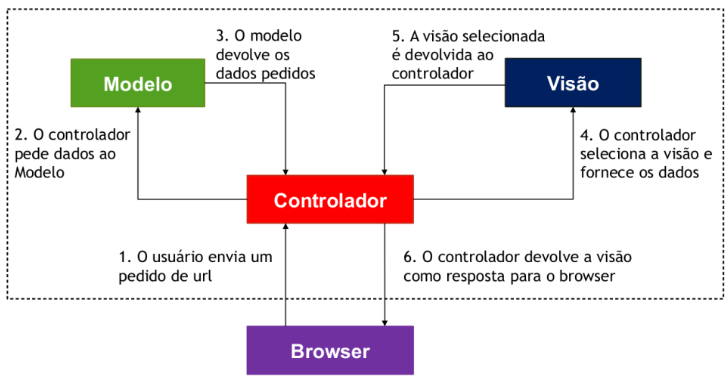
\includegraphics[width=5.0in]{Images/18MVC.png}
    \label{fig: grafico-acc}
    
    \centering \small Fonte: Bruno Lopes, blog Vai de Grails.
\end{figure}

São camadas que auxiliam para facilitar na manutenção, reuso de códigos em outros projetos. \textit{Model} será a camada destinada a modelar as entidades do sistema e manipulação com o banco de dados, responsável pela leitura e escrita de dados, \cite{Gamma2007}. \textit{View} servirá para exibição de dados da interface, permitindo a interação do usuário com o sistema, sendo as informações exibidas em tela. E a camada \textit{Controller} será responsável por controlar e interpretar as informações recebidas e requisições feitas pelo usuário, também responsável pela integração com as camadas \textit{Model} e \textit{View}, \cite{Wazlawick2013}.

O objetivo de se utilizar essa arquitetura de sistema é que ela é simples, facilitando na utilização da linguagem \textit{PHP} e \textit{Javascript} a fazerem as utilizações corretas das camadas, não tendo muitos requisitos de utilização comparado a outros padrões de projetos.


% %%%%%%%%%%%%%%%%%%%%%%%%%%%%%%%%%%%%%%%%%%%%%%%%%%%%%%%%
% %                      4.5                             %
% %%%%%%%%%%%%%%%%%%%%%%%%%%%%%%%%%%%%%%%%%%%%%%%%%%%%%%%%

%04-05-03-01-Revisto[OK]
\section{Materiais utilizados no desenvolvimento do sistema \textit{web}}

Nesta seção serão expostos às técnicas e ferramentas utilizadas durante o desenvolvimento do sistema \textit{website}. A construção de todo o sistema foi a partir da elaboração dos requisitos de sistema, juntamente através do análise do fluxo do usuário e do diagrama de caso de uso permitiram a melhor visualização de funcionalidades a serem construídas. E também se valeu de conhecimento adquirido durante a graduação, de pesquisas realizadas e cursos \textit{online}, que contribuíram para várias etapas no desenvolvimento.

A escolha da linguagem e tecnologias a serem utilizadas foram pensadas e repensadas, visto que foram analisados vários pontos como: manutenção, escalabilidade, baixa complexidade, facilidade na adição de novas funcionalidades, desempenho em requisição, custos, etc.
Outro ponto analisado foi em qual plataforma seria ideal para a construção do sistema, se seria aplicação \textit{mobile}, \textit{desktop} ou \textit{web}, colocando os critérios de escolha: custos para funcionamento, agilidade no desenvolvimento e facilidade para o usuário.

E analisados os pontos elencados acima, a escolha foi de utilizar um sistema \textit{web}, com as telas responsivos, funcionando em um navegador de internet no computador ou celular. Já para as linguagens de programação escolhidas foram o PHP e o Javascript, vistos que ambos têm muitas documentações e funcionalidades que facilitam para o desenvolvedor utilizar.

Na construção de sistemas de \textit{website}, o sistema operacional, os requisitos do sistema, os \textit{hardwares} podem ser qualquer um, sendo de escolha do desenvolvedor, não impactando no desenvolvimento, visto que a construção de uma aplicação \textit{web} são geralmente mais leves. Visto isso, o sistema foi realizado em alguns módulos usando o padrão MVC, sendo a aplicação \textit{web} dividido em duas partes fundamentais: \textit{frontend} e \textit{backend}.  
 
O \textit{frontend} é responsável por interpretar as informações vindas do servidor e demonstrar visualmente para o usuário. Em resumo, é a parte visual de um sistema, onde se utilizam elementos gráficos que permitem ao usuário interagir com os elementos dispostos em tela \cite{Alura}. Já para o \textit{backend}, suas atribuições são de manter as regras de negócio de uma aplicação, como um simples exemplo, seria o encarregado em fazer o controle de acesso de usuários, verificando se a senha está correta ou incorreta \cite{Rocketseat}.

Para a codificação do sistema foi utilizado o editor de código gratuíto \textit{Visual Studio Code} distribuído pela empresa Microsoft. Para a utilização da linguagem PHP foi necessário a instalação da ferramenta Xampp, sendo um pacote que permite utilizar funcionalidades do Apache e para banco de dados o \textit{PHPMyAdmin}. Como controle de versões do código foi utilizado a ferramenta GIT e a plataforma \textit{Github} para hospedar os códigos e diagramas realizados. 

Para esse trabalho, foi escolhido o sistema de gerenciamento de conteúdo  Wordpress. Sendo usado para a construção do guia de orientação de implementação da LGPD do referido trabalho. Visto que o Wordpress permite a agilidade na construção de aplicações \textit{web}, utilização da linguagem PHP, além de vários recursos disponibilizados em bibliotecas de desenvolvimento como: \textit{plugins}, construtor de temas, gerenciamento de postagens, entre outras funcionalidades.

\begin{figure}[ht]
    \centering
    \caption{Painel do Wordpress Dados LGPD.}
    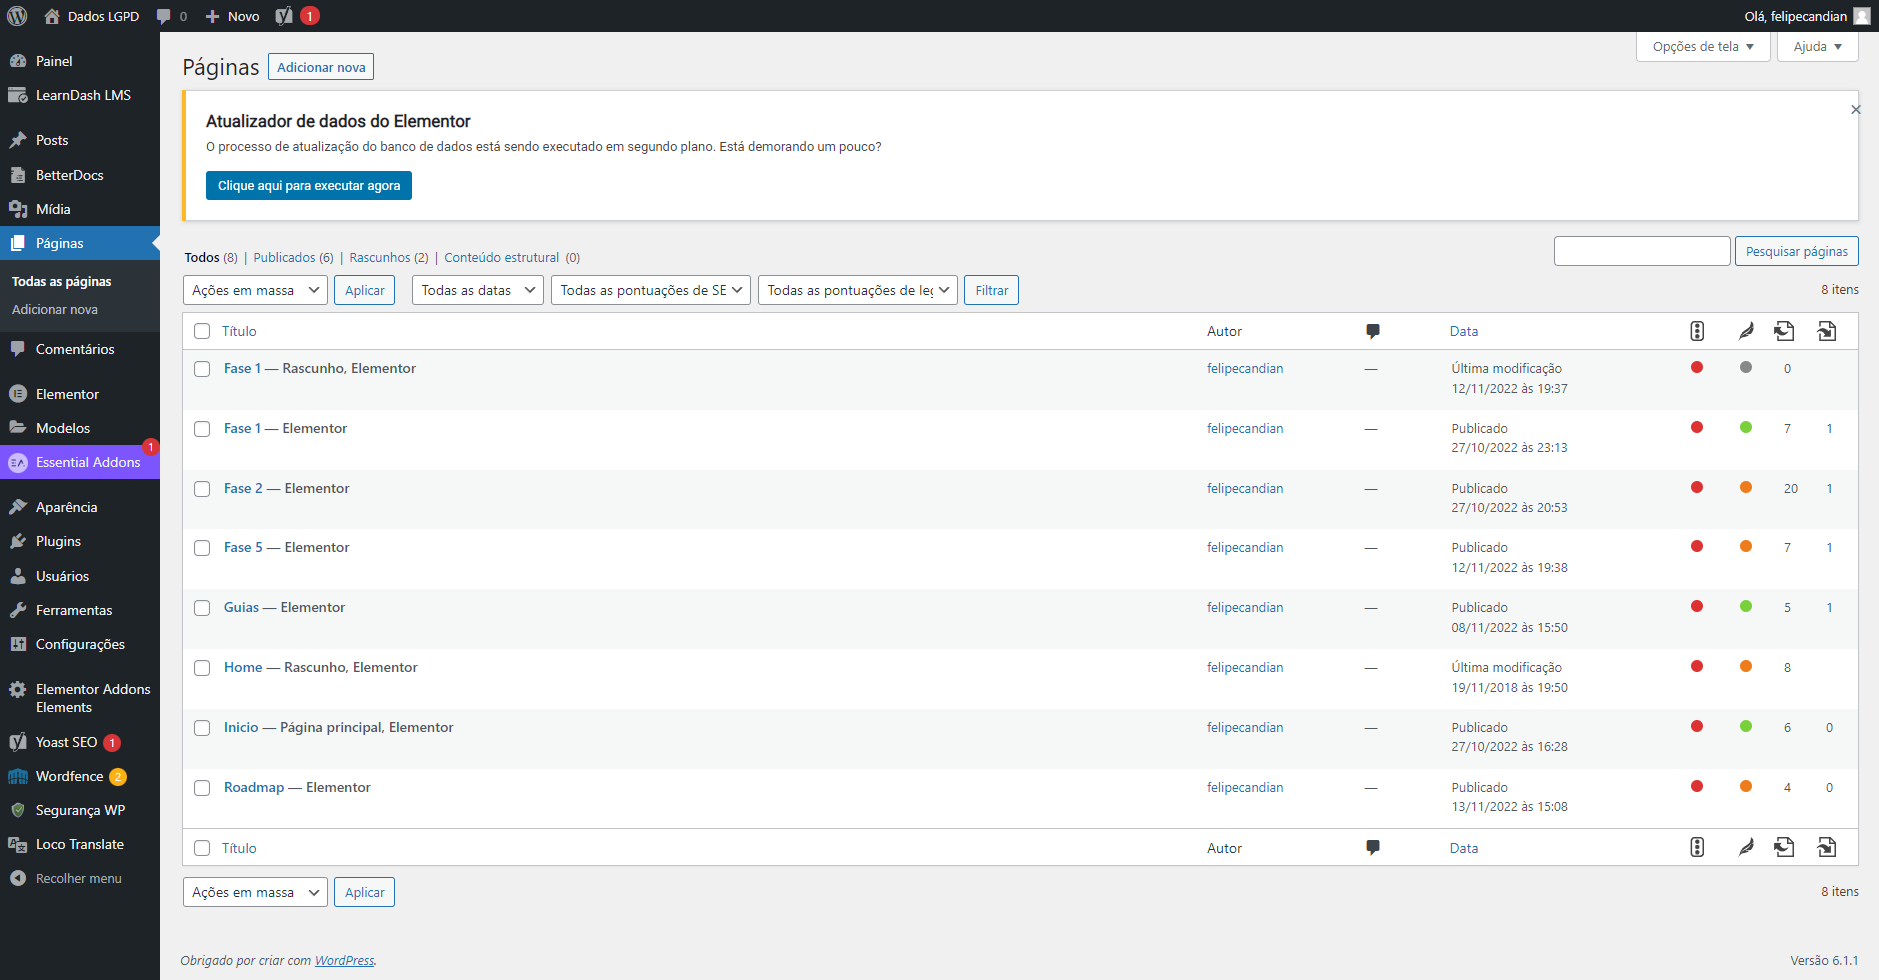
\includegraphics[width=6.0in]{Images/wordpress.png}
    \label{fig: grafico-acc}
    
    \centering \small Fonte: Painel do Wordpress do autor.
\end{figure}

Para colocar a aplicação \textit{web} no ar é necessário utilizar um servidor de hospedagem para \textit{sites}. Neste caso, foi adquirido um servidor com um painel administrativo denominado Cpanel, que já vem pré-configurado pelo serviço de hospedagem para utilizar as ferramentas da linguagem PHP e Apache. Bastou apenas subir os arquivos do Wordpress pelo gerenciador de arquivos  e configurar o banco de dados pelo \textit{PHPMyAdmin}. Na próxima seção será explicado o passo-a-passo para construção do \textit{frontend} e \textit{backend} do \textit{framework}. 
% %%%%%%%%%%%%%%%%%%%%%%%%%%%%%%%%%%%%%%%%%%%%%%%%%%%%%%%%
% %                      4.6                             %
% %%%%%%%%%%%%%%%%%%%%%%%%%%%%%%%%%%%%%%%%%%%%%%%%%%%%%%%%
\section{Construção do \textit{framework} }


Visto os trabalhos relacionados que auxiliaram ao entendimento de projetos com a mesma linha de pensamento, auxiliou bastante com ideias de funcionalidades a serem construídos, juntamente com os requisitos de funcionalidade do sistema já elaborado para o \textit{framework} proposto. Também o livro da coordenadora Viviane Maldonado: LGPD Manual de implementação ajudou na elaboração de fases e etapas.
O \textit{framework web} foi desenvolvido em duas partes: \textit{backend} e \textit{frontend}.  

A construção do \textit{backend} foram realizadas em módulos, sendo a parte de PHP ficou responsável pelo gerenciamento do sistema de questionário do \textit{framework} de implementação. Foi utilizado para sistema de gerenciamento de banco de dados \textit{PHPMyAdmin} em ambiente de produção.

Para o \textit{frontend} foram desenvolvidos várias telas para facilitar a utilização do usuário. Para acessar o \textit{framework web} basta acessar o site:  \url{https://home.felipecandian.com/lgpd/}.
O usuário ao acessar o site do \textit{framework} terá a seguinte página de início conforme a figura abaixo:

\begin{figure}[ht]
    \centering
    \caption{Homepage do \textit{framework} Dados LGPD}
    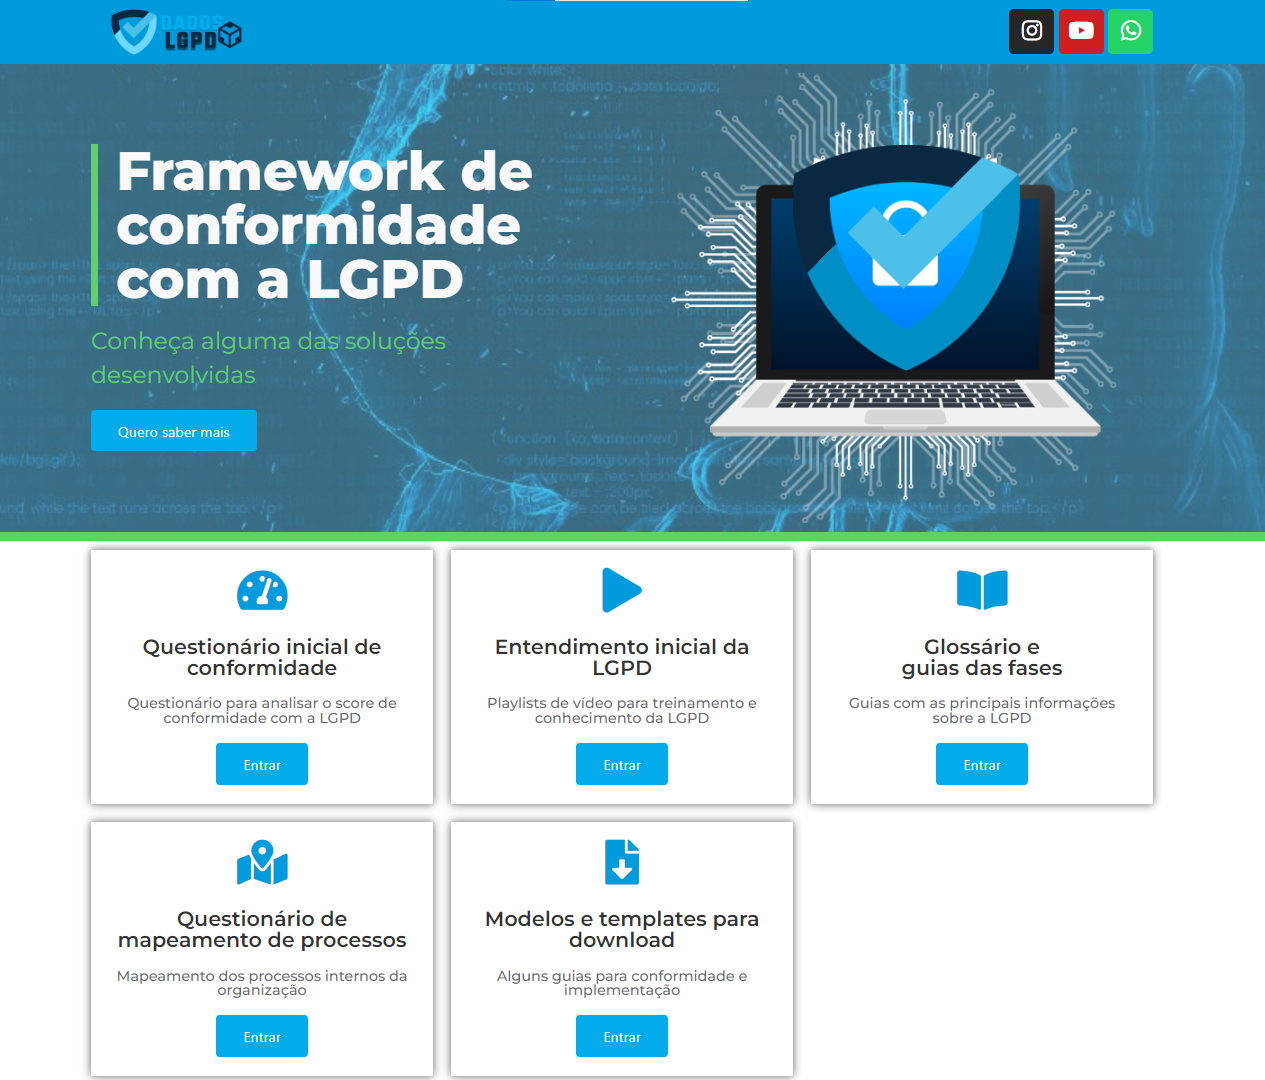
\includegraphics[width=4.0in]{Images/homepag.png}
    \label{fig: homepage}
    
    \centering \small Fonte: Autor.
\end{figure}

Acessando a primeira opção, "Questionário Inicial de conformidade", o usuário será redirecionado ao painel com questionar de conformidade. Bastando ele escolher qual dos questionários disponíveis ele planeja responder, conforme a figura abaixo:

\begin{figure}[ht]
    \centering
    \caption{Questionário de conformidade Dados LGPD}
    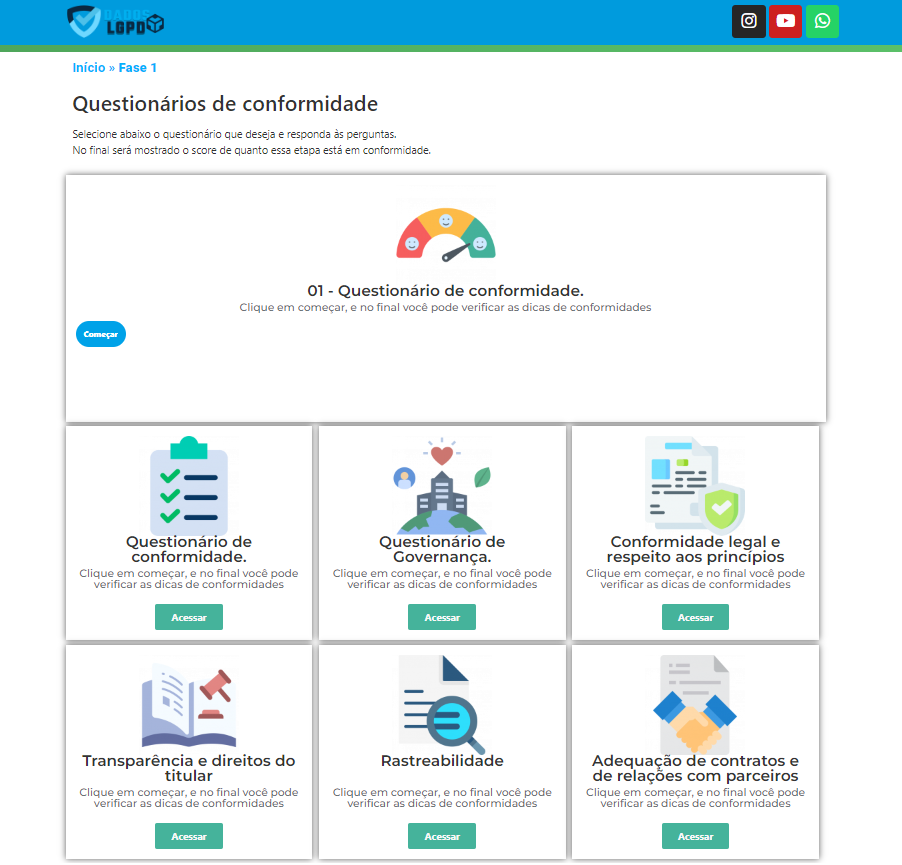
\includegraphics[width=6.6in]{Images/fase1.png}
    \label{fig: homepage}
    
    \centering \small Fonte: Autor.
\end{figure}

Nesta mesma tela, o usuário, escolhendo o questionário desejado, será redirecionado a uma página para ele responder às questões referentes as etapas de adequação com a LGPD, conforme a figura \ref{fig: fase11}. E após responder às questões e submetendo para o sistema, será retornado o porcentual de conformidade, e quais seriam as partes que devem ser adequadas e modificadas caso não esteja em conformidade.


\begin{figure}[ht]
    \centering
    \caption{Questionário de conformidade com as perguntas}
    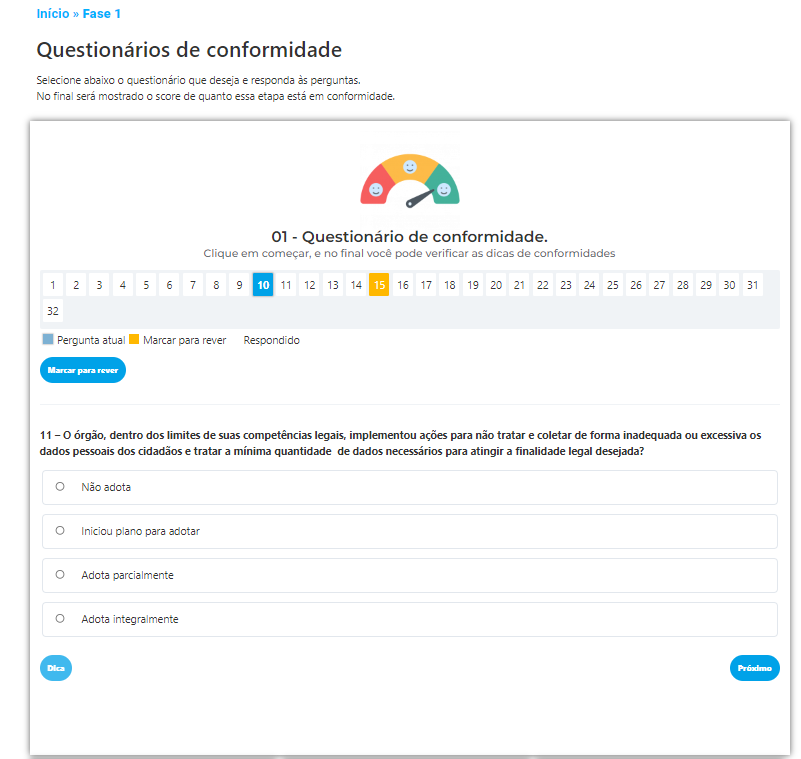
\includegraphics[width=6.2in]{Images/fase11.png}
    \label{fig: fase11}
    
    \centering \small Fonte: Autor.
\end{figure}

O \textit{score} do resultado final será fornecido no final, sendo calculado pelo sistema, sendo o resultante do peso total das perguntas dividido pela quantidade de perguntas. Por exemplo: O questionário tem 10 perguntas, e o peso é 10 para cada resposta certa. O usuário têm em suas respostas 8 questões em conformidade, logo o resultado final será um \textit{score} de 80.

Conforme o cálculo do \textit{score} de conformidade é realizado a partir da seguinte fórmula \ref{eq: score}: 

\begin{equation}
\label{eq: score}
    score = \frac {\textit{peso total das perguntas}} {\textit{quantidade de pergunta}}
\end{equation}

\pagebreak

Conforme a imagem abaixo, após o usuário responder todas as questões, será retornado pelo sistema o \textit{score} e também as sugestões de ações a serem realizadas quando não estiver em conformidade:
\begin{figure}[ht]
    \centering
    \caption{Resultado de exemplo de \textit{score} do conformidade }
    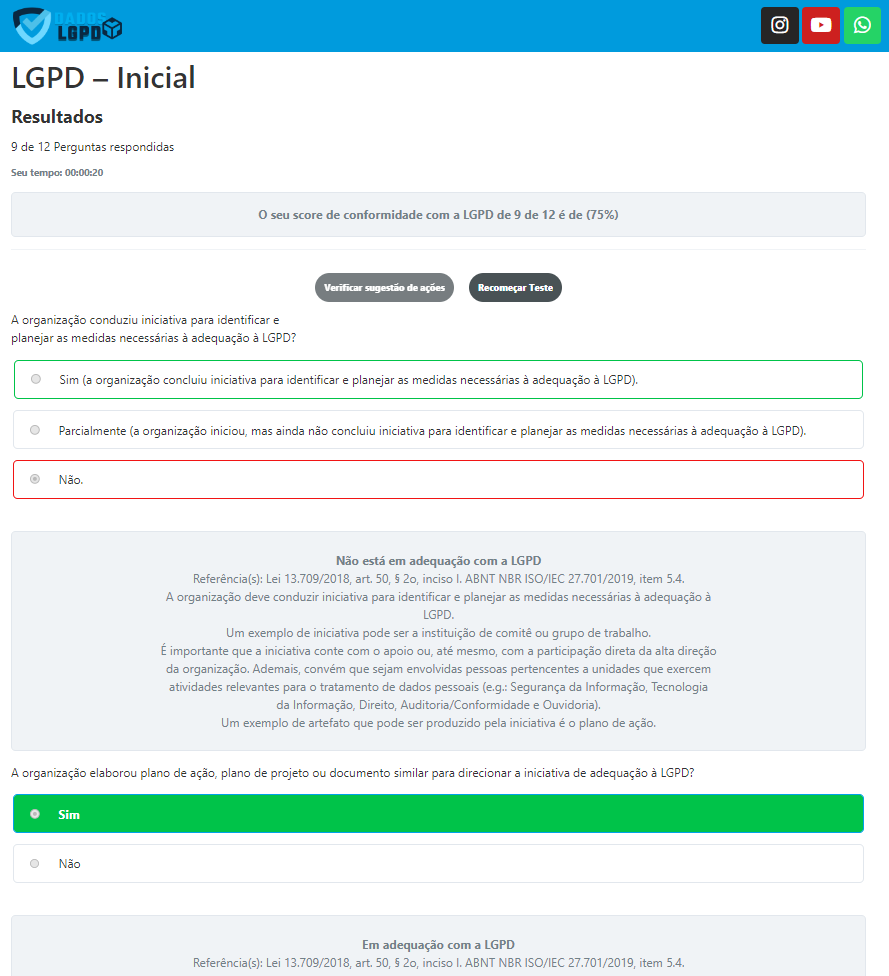
\includegraphics[width=6.8in]{Images/resultado.png}
    \label{fig: resultado}
    
    \centering \small Fonte: Autor.
\end{figure}

\pagebreak

Outra ferramenta para o usuário do \textit{framework} Dados LGPD são os \textit{playlists} de vídeos selecionados para treinamento para usuários que não conhecem profundamente a Lei Geral de Proteção de Dados. Os tópicos dos vídeos são vídeos curtos feitos por terceiros que já estão disponíveis na plataforma Youtube.
A ferramenta está disponível pelo link direto \url{https://home.felipecandian.com/lgpd/fase-2/}, e abaixo a imagem da ferramenta:

\begin{figure}[ht]
    \centering
    \caption{Vídeos de treinamento Dados LGPD}
    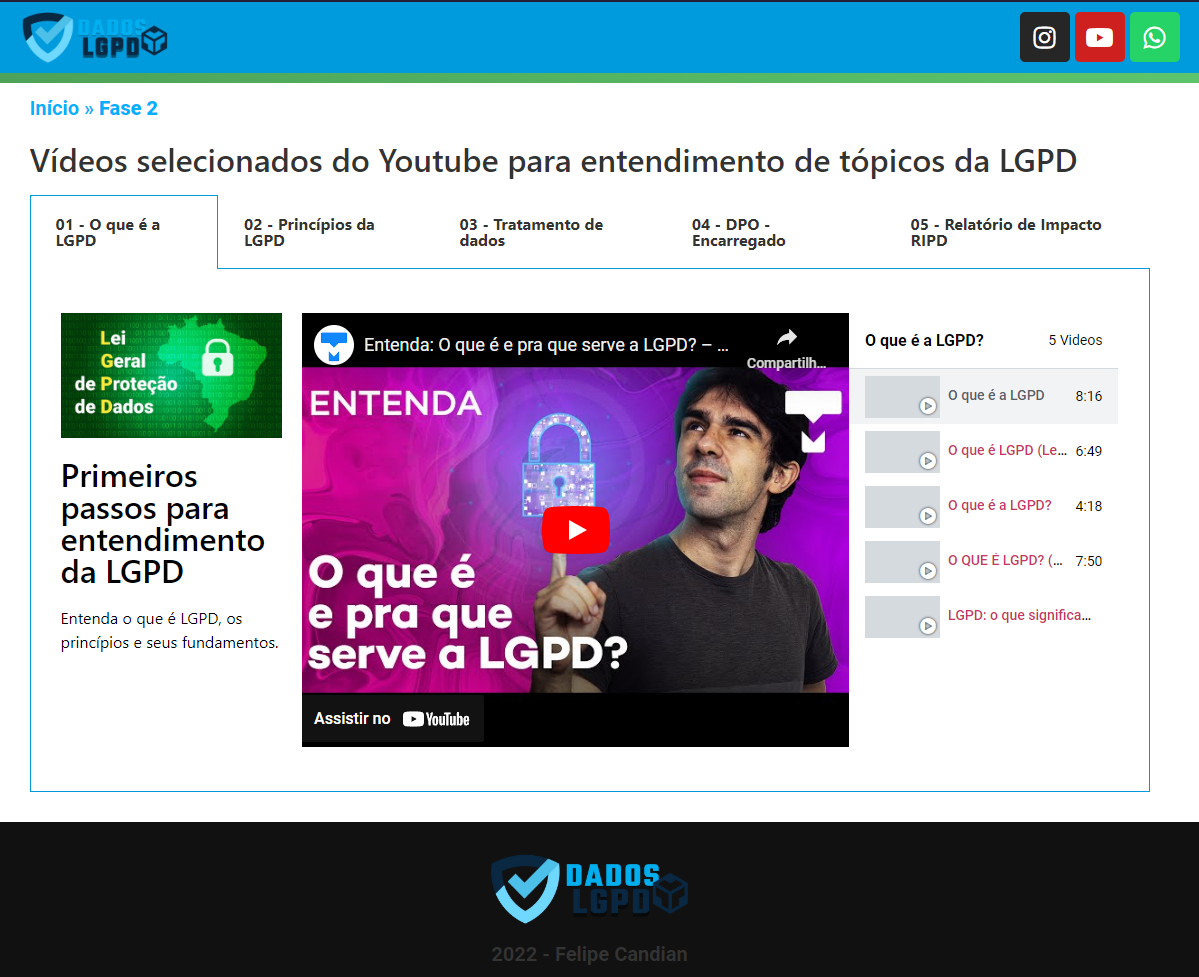
\includegraphics[width=6.5in]{Images/fase2.png}
    \label{fig: workshop}
    
    \centering \small Fonte: Autor.
\end{figure}

Para aprofundar o conhecimento do usuário foi criado o glossário e guia LGPD. Para a criação do guia foi usado o \textit{plugin} BetterDocs que facilitou na criação de documentações que auxiliaram o usuário a ter acesso a textos e notícias que serão uteis durante o processo de conformidade com a lei. 

\pagebreak

Os principais tópicos do guia são os princípios e hipóteses de tratamento, os \textit{frameworks} e \textit{isos} para conformidade com a LGPD, as fases de implementação, o glossário com os termos mais comuns, tabela comparativa entre os artigos.

Essa ferramenta facilitará para o usuário encontrar informações complementares a referida lei. Além de contar com um buscador que poderá facilitar na busca da palavra-chave desejada a ser encontrada e com a possibilidade de imprimir o texto.

O \textit{design} é simples, visando ser intuitivo para o usuário, podendo escolher a categoria do tópico. O guia pode ser acessado pelo link \url{https://home.felipecandian.com/lgpd/guias/}. Abaixo a figura \ref{fig: guiaframe} com a tela quando acessado o guia. 

\begin{figure}[ht]
    \centering
    \caption{Guias com as principais informações sobre a LGPD}
    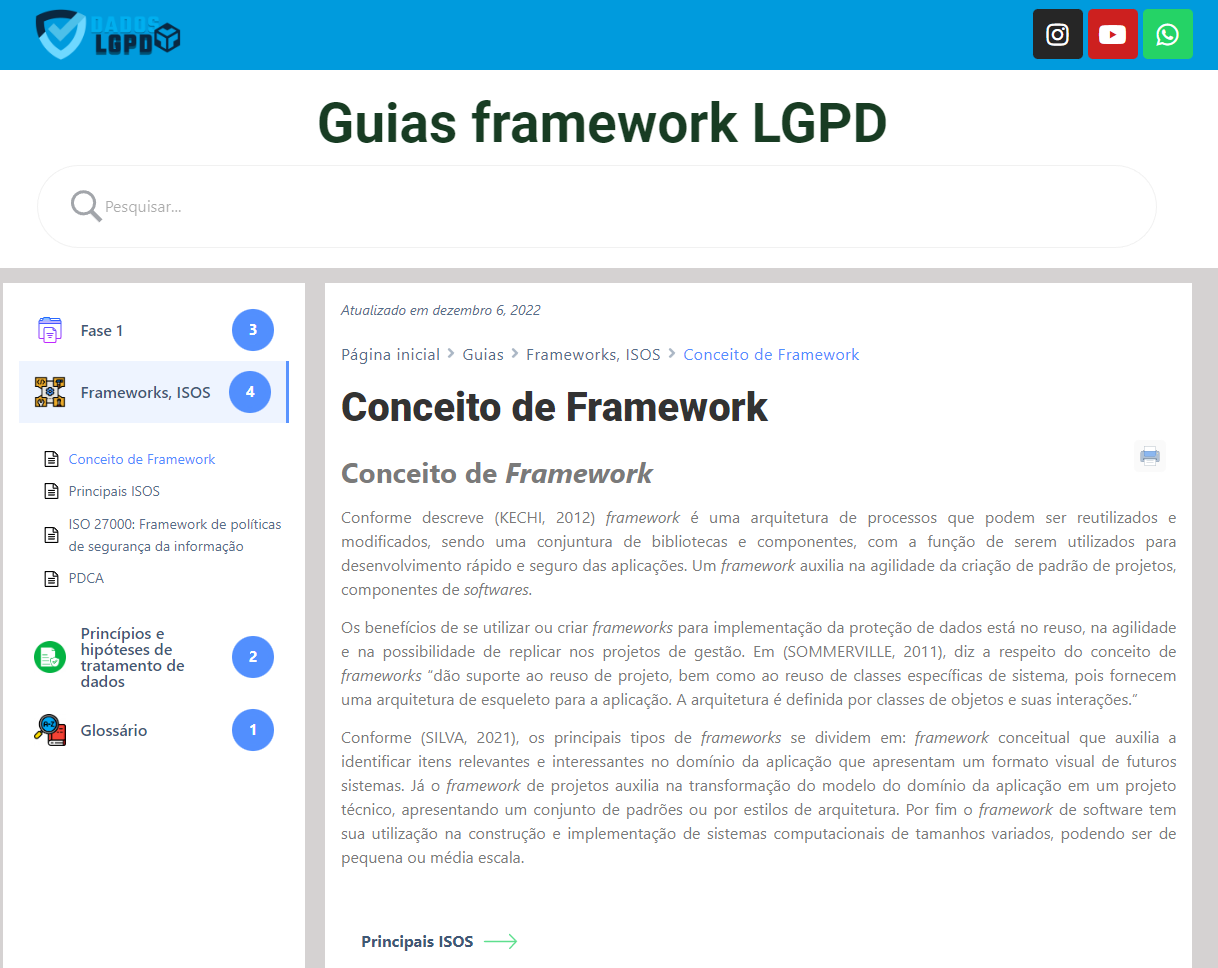
\includegraphics[width=6.0in]{Images/faseglossario.png}
    \label{fig: guiaframe}
    
    \centering \small Fonte: Autor.
\end{figure}

E para facilitar, os encarregados que sempre lidam com documentações no seu dia-a-dia, foi elaborado a página para download de planilhas e guias referente a LGPD. Com essa ferramenta o usuário poderá baixar e modificar planilhas para a etapa que ele estiver do processo de conformidade. Para acessar basta entrar no link e terá acesso ao documento que deseja acessar \url{https://home.felipecandian.com/lgpd/fase-5/}, e abaixo a figura \ref{fig: download} de como ficou visualmente a página:

\begin{figure}[ht]
    \centering
    \caption{Download de planilhas e guias}
    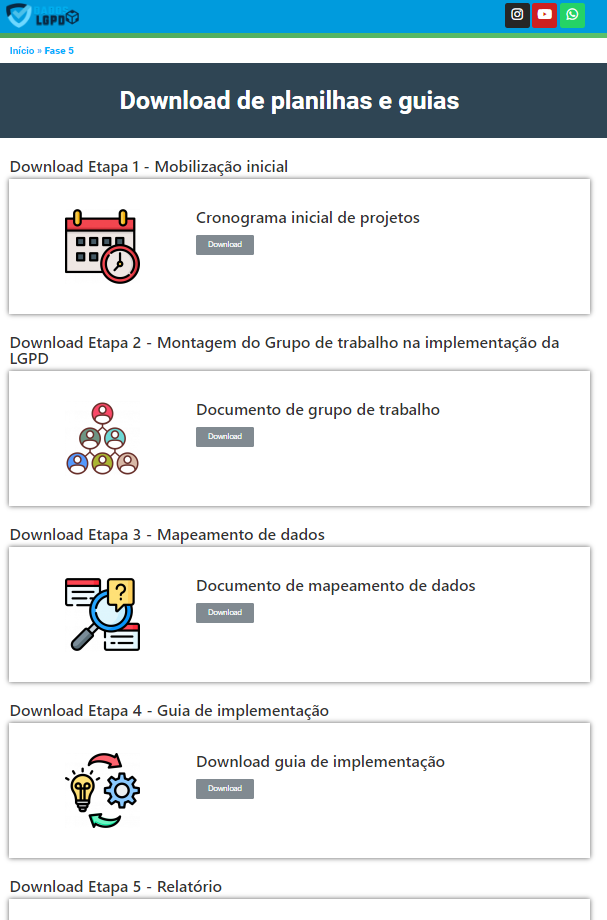
\includegraphics[width=5.0in]{Images/download de planilha.png}
    \label{fig: download}
    
    \centering \small Fonte: Autor.
\end{figure}

\pagebreak
% %%%%%%%%%%%%%%%%%%%%%%%%%%%%%%%%%%%%%%%%%%%%%%%%%%%%%%%%
% %                      4.7                           %
% %%%%%%%%%%%%%%%%%%%%%%%%%%%%%%%%%%%%%%%%%%%%%%%%%%%%%%%%
%\section{Fases do \textit{framework} de conformidade com a LGPD}
%\subsection{Fase I - Preparação para início do processo de conformidade}
%\subsection{Fase II - Análises de \textit{gaps} }
%\subsection{Fase III - Organização do Mapeamento de fluxos de dados e Riscos}
%\subsection{Fase IV - Plano de ação}
%\subsection{Fase V - Treinamento}
%\subsection{Fase VI - Criação de documentos de conformidade}
%\subsection{Fase VII - Execução das ações de conformidade e monitoramento}

%%%%%%%%%%%%%%%%%%%%%%%%%%%%%%%%%%%%%%%%%%%%%%%%%%%%%%%%
%                      Capítulo 5                      %
%%%%%%%%%%%%%%%%%%%%%%%%%%%%%%%%%%%%%%%%%%%%%%%%%%%%%%%%

\chapter{RESULTADOS}
\label{ch: resultados} 

Nessa seção será descrito os resultados obtidos através da avaliação do sistema com os usuários. A pesquisa de avaliação foi feita entre novembro de 2022 e janeiro de 2023, sendo respondido por 25 voluntários que fizeram os testes de usabilidade no site e depois responderam o formulário de avaliação via \textit{Google Forms}. A divulgação do formulário foi realizada por meio de grupos de redes sociais como Facebook e Linkedin, e também em grupos de serviços de mensagens instantâneas Whatsapp e Telegram voltadas a profissionais de proteção de dados e privacidade. O resultado do questionário são apresentadas na próxima seção.

\section{Questionário de avaliação do \textit{framework} }
Com o objetivo de mensurar se o \textit{framework} atende a necessidade dos usuários, e também se contribui durante o processo de conformidade da organização com à LGPD foi criado um formulário no Google \textit{Forms} para avaliar o sistema \textit{framework} desenvolvido. 

O questionário de avaliação está dividido em 2 seções de perguntas. O primeiro conjunto trata do perfil dos participantes e suas experiências. O segundo conjunto trata do quão útil cada etapa do guia é para alcançar a conformidade legal. Ao todo foi realizado 12 perguntas de rápida resposta usando \textit{radio button} e \textit{checkbox}.  O questionário de avaliação está disponível em: \url{https://github.com/felipecandian/TCC-DadosLGPD/tree/main/ANEXOS}.
 
 \subsection{Resposta do questionário: 1ª seção - Perfil do avaliador}
 Na primeira seção foram realizadas perguntas com objetivo de conhecer o avaliador de forma anonima, sendo informado as seguintes informações: "Qual sua faixa etária?", "Qual sua formação acadêmica?", "Qual a sua área de atuação?", "Qual o seu nível de conhecimento na utilização de softwares (programas de computador)?", "Qual o seu nível de familiaridade com a Lei Geral de Proteção de Dados?", "Já usou ou conhece algum desses software para conformidade para LGPD?".
\pagebreak
 
\label{sec: resultados}

\begin{figure}[ht]
    \centering
    \caption{Avaliação.}
    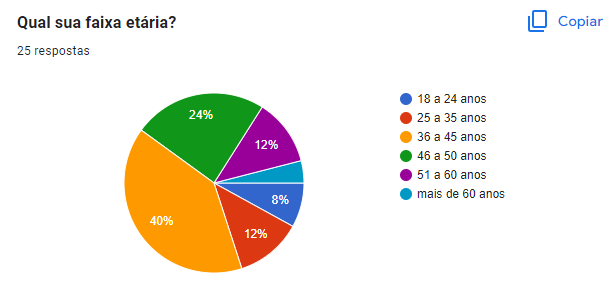
\includegraphics[width=4.0in]{Images/questionario/1.png}
    \label{fig: grafico-acc}
    
    \centering \small Fonte: Autor.
\end{figure}




 \subsection{Resposta do questionário: 2ª seção - Perfil do avaliador}







%%%%%%%%%%%%%%%%%%%%%%%%%%%%%%%%%%%%%%%%%%%%%%%%%%%%%%%%
%                      Capítulo 6                      %
%%%%%%%%%%%%%%%%%%%%%%%%%%%%%%%%%%%%%%%%%%%%%%%%%%%%%%%%
 \chapter{CONCLUSÃO}
 \label{ch: conclusao}
 O \textit{framework} traz inúmeros benefícios às empresas usuárias que necessitam entrar em conformidade, fazendo com que a organização possa entrar em conformidade com a LGPD, bastando que o \textit{DPO}, o encarregado, siga o passo a passo do \textit{framework} exposto neste trabalho. O Dados LGPD é uma ferramenta acessível, com telas de fácil experiência do usuário, fomentando o uso de forma intuitiva, dando um relatório detalhado do percentual do score de conformidade. Conforme apresentado no presente trabalho, foi utilizado as ferramentas Wordpress e \textit{Elementor Builder} com objetivo de usar todo o potencial que o PHP pode proporcionar, como a escalabilidade, facilidade de modificação, atualização, evolução do \textit{software}, reaproveitamento de código através da arquitetura MVC, e as dependências desses \textit{framework} sempre são atualizados, sendo uma grande vantagem. Com a utilização da ferramenta de \textit{framework} gerada nesse trabalho, poderá fazer com que as empresas façam todo o \textit{compliance}, adequando se a lei, e evitando tomar multas que podem desestabilizar a empresa.

Trabalhos futuros serão importantes e valorosos, para mostrar o andamento com o tempo e a aplicação da lei. O \textit{\textit{framework} } DadosLGPD desempenha um papel fundamental para evitar que empresas usem dados pessoais de forma ilegítima de seu banco de dados, e por fim garantindo a privacidade e segurança de seus usuários.



%%%%%%%%%%%%%%%%%%%%%%%%%%%%%%%%%%%%%%%%%%%%%%%%%%%%%%%%
%                      REFERÊNCIAS                     %
%%%%%%%%%%%%%%%%%%%%%%%%%%%%%%%%%%%%%%%%%%%%%%%%%%%%%%%%

% ---
% Finaliza a parte no bookmark do PDF, para que se inicie o bookmark na raiz
% ---
\bookmarksetup{startatroot}% 
% ---

% ---------------------------------------------------------------------------------------------
% ELEMENTOS PÓS-TEXTUAIS
% ---------------------------------------------------------------------------------------------
\postextual


% ---------------------------------------------------------------------------------------------
% Referências bibliográficas
% ---------------------------------------------------------------------------------------------
\bibliography{abntex2-modelo-references}

% ---------------------------------------------------------------------------------------------
% Glossário
% ---------------------------------------------------------------------------------------------
%
% Consulte o manual da classe abntex2 para orientações sobre o glossário.
%
%\glossary

% ---------------------------------------------------------------------------------------------

% Anexos
% ---------------------------------------------------------------------------------------------

% ---
% Inicia os anexos
% ---
%\begin{anexosenv}

% Imprime uma página indicando o início dos anexos
%\partanexos

%\chapter{Protocolo de Aquisição de Imagens}

%\end{anexosenv}

% ---------------------------------------------------------------------------------------------
% INDICE REMISSIVO
% ---------------------------------------------------------------------------------------------

\printindex

\end{document}
